%%
%% This is file `sample-sigconf.tex',
%% generated with the docstrip utility.
%%
%% The original source files were:
%%
%% samples.dtx  (with options: `sigconf')
%% 
%% IMPORTANT NOTICE:
%% 
%% For the copyright see the source file.
%% 
%% Any modified versions of this file must be renamed
%% with new filenames distinct from sample-sigconf.tex.
%% 
%% For distribution of the original source see the terms
%% for copying and modification in the file samples.dtx.
%% 
%% This generated file may be distributed as long as the
%% original source files, as listed above, are part of the
%% same distribution. (The sources need not necessarily be
%% in the same archive or directory.)
%%
%% The first command in your LaTeX source must be the \documentclass
%% command.
\documentclass[sigconf,review, anonymous]{acmart}
\acmConference[ESEC/FSE 2020]{The 28th ACM Joint European Software Engineering Conference and Symposium on the Foundations of Software Engineering}{8 - 13 November, 2020}{Sacramento, California, United States}

\pagenumbering{arabic} % Remove for camera-ready

\usepackage{subcaption}
\usepackage{libertine}
\usepackage{lipsum}% http://ctan.org/pkg/lipsum
\usepackage{algorithm}% http://ctan.org/pkg/algorithm
\usepackage{algpseudocode}% http://ctan.org/pkg/algorithmicx
\usepackage{graphicx}
\usepackage[compatibility=false]{caption}% http://ctan.org/pkg/caption
\usepackage{booktabs}
%% \usepackage{cite}
\usepackage{url}
\usepackage{multirow}
\usepackage{pgfplots}
\usepackage{tikz}
\usetikzlibrary{matrix,fit,shapes,calc,positioning,shadows,arrows,shapes,backgrounds,decorations.markings,fadings}
\usepackage{listings}
%\usepackage[caption=false, font=footnotesize]{subfig}
\renewcommand{\ttdefault}{pcr}
\lstset{
  basicstyle=\scriptsize\ttfamily,
  keywordstyle=\scriptsize\ttfamily\bfseries,
  language=C,             % choose the language of the code
  frame=single,              % adds a frame around the code
  aboveskip=0pt,
  belowskip=0pt,
  breaklines=true,           % sets automatic line breaking
  breakatwhitespace=true,   % sets if automatic breaks should only happen at
  showspaces=false,
  %numbersep=5pt,              % Abstand der Nummern zum Text
  %tabsize=2,                  % Groesse von Tabs
  %extendedchars=true,         %
  keywords=[2]{tcp, flag, threshold, track, count, seconds, classtype, sid}
}
\usepackage{balance}
\usepackage{wrapfig}
\usepackage{enumitem}
\usepackage{color, colortbl}
\definecolor{Gray}{gray}{0.9}
\usepackage[skins]{tcolorbox}

%% 
\newcommand{\tname}{\textsc{Syrius}} %% name of the technique
\newcommand{\ie}{i.e.}
\newcommand{\eg}{e.g.}
\newcommand{\aka}{a.k.a.}
\newcommand{\etal}{and colleagues}
\newcommand{\nids}{NIDS}
\newcommand{\metas}{Metasploit}
\newcommand{\suri}{Suricata}
\newcommand{\numrulessuri}{27.8K}
\newcommand{\percRulesWithContent}{93.5\%}
\newcommand{\numundetected}{\Fix{XX\%}}
\newcommand{\CodeIn}[1]{{\small{\texttt{#1}}}}
\newcommand{\MyComment}[1]{}

%% review
\newcommand{\Fix}[1]{{\textbf{[[}\color{magenta}#1}\textbf{]]}}
\newcommand{\Mar}[1]{{\textbf{[[Marcelo:~}\color{red}#1}\textbf{]]}}
\newcommand{\Luc}[1]{{\textbf{[[Lucas:~}\color{blue}#1}\textbf{]]}}
\newcommand{\Gui}[1]{{\textbf{[[Guilherme:~}\color{green}#1}\textbf{]]}}

\def\denseitems{
   \itemsep1pt plus1pt minus1pt
   \parsep0pt plus0pt
   \parskip0pt\topsep0pt}

%% numbers
\newcommand{\totoptions}{162}
\newcommand{\numproto}{11}
\newcommand{\totoptionsrelevant}{153}


%%
%% \BibTeX command to typeset BibTeX logo in the docs
\AtBeginDocument{%
  \providecommand\BibTeX{{%
    \normalfont B\kern-0.5em{\scshape i\kern-0.25em b}\kern-0.8em\TeX}}}

%% Rights management information.  This information is sent to you
%% when you complete the rights form.  These commands have SAMPLE
%% values in them; it is your responsibility as an author to replace
%% the commands and values with those provided to you when you
%% complete the rights form.
%% \setcopyright{acmcopyright}
%% \copyrightyear{2018}
%% \acmYear{2018}
%% \acmDOI{10.1145/1122445.1122456}

%% These commands are for a PROCEEDINGS abstract or paper.
%% \acmConference[Woodstock '18]{Woodstock '18: ACM Symposium on Neural
%%   Gaze Detection}{June 03--05, 2018}{Woodstock, NY}
%% \acmBooktitle{Woodstock '18: ACM Symposium on Neural Gaze Detection,
%%   June 03--05, 2018, Woodstock, NY}
%% \acmPrice{15.00}
%% \acmISBN{978-1-4503-XXXX-X/18/06}


%%
%% Submission ID.
%% Use this when submitting an article to a sponsored event. You'll
%% receive a unique submission ID from the organizers
%% of the event, and this ID should be used as the parameter to this command.
%%\acmSubmissionID{123-A56-BU3}

%%
%% The majority of ACM publications use numbered citations and
%% references.  The command \citestyle{authoryear} switches to the
%% "author year" style.
%%
%% If you are preparing content for an event
%% sponsored by ACM SIGGRAPH, you must use the "author year" style of
%% citations and references.
%% Uncommenting
%% the next command will enable that style.
%%\citestyle{acmauthoryear}

%%
%% end of the preamble, start of the body of the document source.
\begin{document}

%%
%% The "title" command has an optional parameter,
%% allowing the author to define a "short title" to be used in page headers.
\title{Learning to Synthesize Rules for Network Intrusion Detectors}

%%
%% The "author" command and its associated commands are used to define
%% the authors and their affiliations.
%% Of note is the shared affiliation of the first two authors, and the
%% "authornote" and "authornotemark" commands
%% used to denote shared contribution to the research.
\author{Ben Trovato}
\authornote{Both authors contributed equally to this research.}
\email{trovato@corporation.com}
\orcid{1234-5678-9012}
\author{G.K.M. Tobin}
\authornotemark[1]
\email{webmaster@marysville-ohio.com}
\affiliation{%
  \institution{Institute for Clarity in Documentation}
  \streetaddress{P.O. Box 1212}
  \city{Dublin}
  \state{Ohio}
  \postcode{43017-6221}
}

\author{Lars Th{\o}rv{\"a}ld}
\affiliation{%
  \institution{The Th{\o}rv{\"a}ld Group}
  \streetaddress{1 Th{\o}rv{\"a}ld Circle}
  \city{Hekla}
  \country{Iceland}}
\email{larst@affiliation.org}

\author{Valerie B\'eranger}
\affiliation{%
  \institution{Inria Paris-Rocquencourt}
  \city{Rocquencourt}
  \country{France}
}

\author{Aparna Patel}
\affiliation{%
 \institution{Rajiv Gandhi University}
 \streetaddress{Rono-Hills}
 \city{Doimukh}
 \state{Arunachal Pradesh}
 \country{India}}

\author{Huifen Chan}
\affiliation{%
  \institution{Tsinghua University}
  \streetaddress{30 Shuangqing Rd}
  \city{Haidian Qu}
  \state{Beijing Shi}
  \country{China}}

\author{Charles Palmer}
\affiliation{%
  \institution{Palmer Research Laboratories}
  \streetaddress{8600 Datapoint Drive}
  \city{San Antonio}
  \state{Texas}
  \postcode{78229}}
\email{cpalmer@prl.com}

\author{John Smith}
\affiliation{\institution{The Th{\o}rv{\"a}ld Group}}
\email{jsmith@affiliation.org}

\author{Julius P. Kumquat}
\affiliation{\institution{The Kumquat Consortium}}
\email{jpkumquat@consortium.net}

%%
%% By default, the full list of authors will be used in the page
%% headers. Often, this list is too long, and will overlap
%% other information printed in the page headers. This command allows
%% the author to define a more concise list
%% of authors' names for this purpose.
\renewcommand{\shortauthors}{Trovato and Tobin, et al.}

%%
%% The abstract is a short summary of the work to be presented in the
%% article.
\begin{abstract}
Network Intrusion Detection Systems (\nids{}) are a popular mechanism
used by system administrators to defend against network attacks. These
systems monitor the network traffic and flag suspicious network
behavior. Signature-based \nids\ do that by checking the\MyComment{ network}
traffic against a pre-defined set of rules, which become obsolete
as attackers learn new strategies to circumvent existing defenses.

This paper proposes \tname{}, a technique that automatically
synthesizes \nids\ rules from positive and negative examples, \ie{},
malicious and benign traffic. \tname{} formulates synthesis as an
optimization problem whose candidate solutions are rules. Optimal
solutions maximize the capture of positive traffic and minimize the
capture of negative traffic. \tname{} bootstraps the search with a
candidate solution inferred from the payload of the malicious message.
It uses that initial overfitting solution to search for alternative
rules that only capture the malicious traffic. Then, it ranks those
rules according to heuristics---drawn from a data set of existing
rules---denoting the likelihood of those rules of being useful.

We evaluated \tname{} on a diverse
set of attacks. Results indicate that \Fix{...}
\end{abstract}

%%
%% The code below is generated by the tool at http://dl.acm.org/ccs.cfm.
%% Please copy and paste the code instead of the example below.
%%
\begin{CCSXML}
<ccs2012>
 <concept>
  <concept_id>10010520.10010553.10010562</concept_id>
  <concept_desc>Computer systems organization~Embedded systems</concept_desc>
  <concept_significance>500</concept_significance>
 </concept>
 <concept>
  <concept_id>10010520.10010575.10010755</concept_id>
  <concept_desc>Computer systems organization~Redundancy</concept_desc>
  <concept_significance>300</concept_significance>
 </concept>
 <concept>
  <concept_id>10010520.10010553.10010554</concept_id>
  <concept_desc>Computer systems organization~Robotics</concept_desc>
  <concept_significance>100</concept_significance>
 </concept>
 <concept>
  <concept_id>10003033.10003083.10003095</concept_id>
  <concept_desc>Networks~Network reliability</concept_desc>
  <concept_significance>100</concept_significance>
 </concept>
</ccs2012>
\end{CCSXML}

\ccsdesc[500]{Computer systems organization~Embedded systems}
\ccsdesc[300]{Computer systems organization~Redundancy}
\ccsdesc{Computer systems organization~Robotics}
\ccsdesc[100]{Networks~Network reliability}

%%
%% Keywords. The author(s) should pick words that accurately describe
%% the work being presented. Separate the keywords with commas.
\keywords{\nids, synthesis, search}

%% This command processes the author and affiliation and title
%% information and builds the first part of the formatted document.
\maketitle

\section{Introduction}
\label{sec:intro}

Network Intrusion Detection Systems (\nids{}) are software systems
that monitor the network traffic for malicious behavior and act
accordingly by blocking messages or alerting humans about suspicious
events~\cite{Mitchell:2014:SID:2597757.2542049}. \nids{} are typically
placed behind a firewall, vetting the traffic that the firewall did
not block. Various open-source (\eg{}, Snort~\cite{snort} and
Suricata~\cite{suricata}) and commercial \nids\ implementations (\eg{},
SolarWinds~\cite{solarwinds} and IBM QRadar~\cite{qradar}) exist
today. These systems are very popular in industry to secure local
computer networks given the amount of potential malicious traffic that
exist on the Internet.

This paper focuses on rule-based \nids{}, which are very popular in
industry~\cite{proofpoint-etpro,snort-rule-subscriptions}. A
\emph{rule-based intrusion detector}\footnote{\aka\ signature-based
  intrusion detector.} checks if the network traffic matches a fixed
set of rules. Figure~\ref{fig:pingscan-example} shows an example rule
of Suricata~\cite{suricata}, a popular open-source \nids{}. This
particular rule prescribes a method to capture an Active
Reconnaissance attack for discovering which ports of a publicly
accessible machine are open for connection. Rulesets exist for
Snort~\cite{snort} and Suricata~\cite{suricata}, providing protection
against existing attacks. Unfortunately, attackers actively look for
new mechanisms to exploit systems. For example, Figure~\Fix{plot}
shows the increase in number of rules added to the ``Emerging Threats
Open Ruleset''---a popular public data set of \suri\ rules---in the
past 12 months.

\Fix{add figure here}

Intuitively, rulesets need to be constantly revised to protect a
system against attackers. Unfortunately, creating these rules is
time-consuming as the language for describing rules is non-trivial
(see Section~\ref{sec:example-suricata-rules}) and it is error-prone
as checking whether the rule captures only malicious traffic is
non-trivial.

%% IT-security companies capitalize on this phenomena and
%% offer rulesets on the
%% market.

This paper proposes \tname{}\footnote{Abbreviation for
  \textbf{Sy}nthesis of Su\textbf{ri}cata R\textbf{u}le\textbf{s}.}, a
technique that uses machine intelligence to automatically synthesize
rules for rule-based \nids. Our goal is to facilitate the creation of
rules and, consequently, harden the protection of \nids\ to network
attacks. \tname{} synthesizes rules from malicious and benign traffic
and from examples of correct rules.

\Fix{
denial-of-service
attack to a server by matching specific conditions about the network
traffic~\cite{understanding-dos}. Relevant properties about the
traffic of interest appear in bold in this rule (see
Section~\ref{sec:suri-metas-coverage}). Deployments of rule-based
\nids\ are restricted to a fixed set of rules defined by the network
system administrator.}\Mar{check...}



%% Note that anomaly-based \nids are evolving pretty quick with the
%% advances in machine learning, but rule-based \nids are still extremely
%% popular.  \tname{} could also leverage existing databases of malicious
%% traffic to synthesize rules.  Regardless of how the negative traffic
%% is produced (out of scope of this paper), those rules can be
%% distributed to rule databases for free.
%%  The
%% core motivation is that 1) attackers are productive in creating new
%% ways to circumvent existing protections and 2) manual creation of
%% rules is tedious and time-consuming.  

\Fix{summarize how the technique works}

\Fix{summarize results} We believe these results provide initial
evidence on the effectiveness of \tname{}.

This paper makes the following contributions.

\section{Network Intrusion Detection Systems (\nids)}
\label{sec:background}

\subsection{Rule-based and Anomaly-based \nids}

\sloppy \nids{} are typically categorized in two
groups~\cite{kumar2007survey}: rule-based (see
Section~\ref{sec:intro}) and anomaly-based \nids. An
\emph{anomaly-based intrusion detector} learn usage behavior from
benign traffic and, based on that, alert uncommon
behavior~\cite{7579764,kumar2007survey,Mitchell:2014:SID:2597757.2542049,cordy-etal-issta19}. More
precisely, an anomaly-based \nids{} flags an attack when the network
traffic manifests different characteristics compared to those of the
benign traffic.

Rule-based \nids\ can miss attacks as rulesets can become outdated
whereas anomaly-based \nids\ can report false alarms as learning
algorithms that generalize observations from bening traffic are
approximate. To sum up, rule-based \nids{} and anomaly-based \nids{}
are complementary---a rule-based \nids{} focuses on known attacks
whereas anomaly-based \nids{} focuses on unknown potential attacks.
This paper focuses on rule-based \nids\ for its tremendous popularity
in industry. Although we focused on the Suricata \nids, the principles
we used are general to any other signature-based \nids~(\eg{},
Snort~\cite{snort}).


\subsection{Suricata Rules}
\label{sec:example-suricata-rules}

Figure~\ref{fig:synflood-example} shows an example rule of
Suricata~\cite{suricata}, a popular open-source \nids{} maintained by
the Open Information Security Foundation (OISF)~\cite{oisf}.
A Suricata rule is divided in three parts---action, header, and rule
options~\cite{suri-rule-format}. The action part appears as the first
word in the rule description. An action denotes the task that needs to
be executed if the rule pattern is satisfied.  In this example, a
message will be sent to system administrators if the rule pattern is
satisfied. The header comes after the action in the rule
description. It restricts the information flow covered by the
rule. The header of this rule is \CodeIn{icmp any any -> any
  any}. It instructs Suricata to inspect \CodeIn{icmp} traffic flowing
from any machine and port to any machine and port.\MyComment{ The variables
\CodeIn{\$HOME\_NET} and \CodeIn{\$EXTERNAL\_NET} are
configurable.} The rule options come after the header. It is a
semi-colon-separated sequence of key-value pairs. Rule options serve
to document the analyzed traffic (\eg{}, ``msg'', ``classtype'', and
``sid'') and to characterize the attack pattern (\eg, ``flags'',
``threshold'', and ``content''). \tname{} produces options of the
second kind, which are \emph{relevant} to capture the attack. For
example, the option \CodeIn{content:<arg>} checks if the argument is
present in the payload of the message.

\vspace{-1ex}
\begin{table}[h!]
  \footnotesize
  \caption{\label{table:rules}Example of non-documentation options of Suricata.}
  \vspace{-2ex}
  \centering
  \begin{tabular}{clp{5.5cm}}
    \toprule
    \multicolumn{1}{c}{\#} & \multicolumn{1}{c}{Name} &  \multicolumn{1}{c}{Description}\\
    \midrule     
    1 & dsize & matches on the size of the packet payload\\
    2 & itype &  matches on a specific ICMP type\\
    3 & icode & matches on a specific ICMP code\\
    4 & icmp\_seq  & checks a ICMP sequence number\\
    5 & icmp\_id & matches on specific ICMP id-values\\
    6 & window & checks the size of the TCP window\\
    7 & flags & matches on TCP flags\\
    8 & fragbits & checks if the fragmentation or reserved bits are set in the IP header\\
    9 & threshold & minimum threshold for a rule before it generates alerts\\
    10 & content & checks if argument is present on the payload\\
    \bottomrule
  \end{tabular}
\end{table}
%\vspace{-1ex}

Table~\ref{table:rules} shows a sample of non-documentation options of
Suricata. Column ``\#'' shows the option number, column ``Name'' shows
the name of the option, and column ``Description'' summarizes
purpose. The option \CodeIn{content} is very common in rules to
capture http attacks, which are the most common kind of rules. This
option takes a sequence of bytes as argument (\eg{},
\CodeIn{content:''SELECT ''}) and checks if that sequence is present
in the payload of the message. Detailed description of the Suricata
rules can be found elsewhere~\cite{suri-rule-format}. It is worth
noting that Suricata supports a total of \totoptions\ distinct options
covering \numproto\ distinct protocols.


%% A total of 9 of these options
%% are for documentation.\MyComment{For instance, the purpose of rule
%%   option \CodeIn{msg} is to print on the output an informative message
%%   indicating what kind of intrusion has been observed.}
%% Figure~\ref{fig:distribution-rules-protocol} shows the distributions
%% of these options per protocol. The sum of the number of protocol
%% options is higher than \totoptions\ as some options are shared across
%% different protocols. \tname{} does not make distinction among protocols.


%% %\begin{wrapfigure}[14]{r}{0.5\textwidth}
%% \begin{figure}[t!]
%%   \centering
%% %  \vspace{-7ex}
%%   \scalebox{0.85}{
%%     \begin{tikzpicture}
%%       \begin{axis}[
%%           ybar stacked,
%%           enlargelimits=0.15,
%%           legend style={at={(0.5,-0.15)},
%%             anchor=north,legend columns=-1},
%%           %          ylabel={\#rules},
%%           symbolic x coords={dns, ftp, http, icmp, ip, smb, smtp, ssh,
%%           tcp, tls, udp},
%%           xtick=data,
%%           xticklabel style={rotate=45},          
%%           nodes near coords,
%%           every node near coord/.append style={font=\scriptsize},        
%%           nodes near coords align={vertical},
%%         ]
%%         \addplot coordinates {(dns,10) (ftp,11) (http,20) (icmp,18)(ip,16) (smb,13) (smtp,11) (ssh, 10) (tcp, 32) (tls,18) (udp, 18)};
%% %        \legend{relevant, irrelevant}
%%       \end{axis}
%%     \end{tikzpicture}
%%   }
%%   \vspace{-2ex}
%%   \caption{\label{fig:distribution-rules-protocol}Number of relevant
%%     options per protocol supported by Suricata.\Mar{not sure if this
%%       is really helpful.}}
%% %\end{wrapfigure}
%% \end{figure}
  

\subsection{Rules and Packets}
\label{sec:rules-and-packets}

Rule options are often associated with specific fields of network
packets. Let's consider the ICMP protocol as an
example. Figure~\ref{fig:icmp-packet-layout} shows the layout of an
ICMP packet. The packet fields ``Flags'' and ``Time to Live'',
declared in the IP header, are mapped to the options \CodeIn{flagbits}
and \CodeIn{ttl}, respectively. Likewise, the fields ``Type'' and
``Code'', declared in the ICMP header, are mapped to the options
\CodeIn{itype} and \CodeIn{icode}. The values of the options ``ttl'',
``itype'', and ``icode'' are the same as the value of the
corresponding fields in the ICMP packet. For the field ``Flags'' the
value of the corresponding option is encoded in a bitvector. For
example, if the ``Flags'' field stores the value 1010, the
corresponding rule option will be \CodeIn{flagbits:RM}, as each
position of the vector encodes a different character in the
\CodeIn{flagbits} rule option. The value of several options can be
determined through transformation functions, as those described
above. One exception to this is the option \CodeIn{threshold}, which
is typically used in denial-of-service attacks. That option operates
over sequence of messages as opposed to a single
message. Consequently, it is not possible to determined its values
from a single message.

\begin{figure}[t!]
\centering
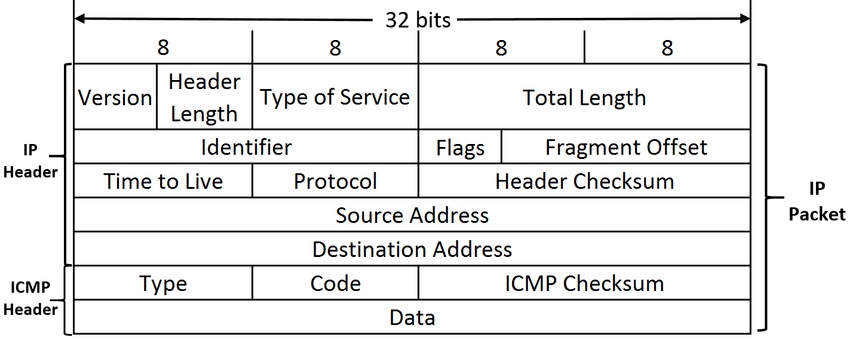
\includegraphics[scale=0.28]{figs/ICMP-packet-structure.png}
\vspace{-2ex}
\caption{Layout of an ICMP packet.}
\label{fig:icmp-packet-layout}
\end{figure}
%\vspace{-2ex}

%% More precisely, to trigger an action on a rule
%% containing that option a \nids\ tool needs to monitor several
%% messages.

%% \Luc{
%%   Os campos Flags e Time to live no header IP são mapeados para as opções fragbits e ttl, respectivamente. Os campos Type e Code no header ICMP são mapeados para as opções itype e icode. \\
%% Os campos, Time to Live, Type e Code recebem diretamente o valor que está no pacote. Por exemplo, se o campo Type no pacote possuir valor 8, na regra ele vai aparecer como itype:8.\\
%% O campo Flags é intepretado como um vetor de bits, onde cada posição representa uma flag. Na regra, o valor do campo Flags é traduzido em caracteres que representam cada flag presente no pacote. Por exemplo: se o campo Flags possuir o valor 1010, na regra aparecerá fragbits:RM, pois os caracteres R e M indicam a presença do quarto e segundo bits.}


\section{Illustrative Example}
\label{sec:suri-metas-coverage}
\label{sec:active-recon}

This section briefly shows how \tname{} synthesizes rules for one
example attack. Active Reconnaissance is a method used by malicious
individuals to collect information about a computing system to
determine potential vulnerabilities. This method is used as a
preliminary step towards an actual attack. For example, Ping Scan
scans the network for IPs of accessible hosts. An attacker sends
several ICMP Echo requests to a range of IP addresses in the network
and checks which ones respond to these requests. This method enables
an attacker to know which machines are active in the network.

%\vspace{-1ex}
\begin{figure}[h!]
  \lstinputlisting[language=C,numbers=none,keywords={dsize,itype}]{pingscan.suricata}
  \vspace{-2ex}  
  \caption{Suricata rule for Ping Scan attack.}
  \label{fig:pingscan-example}
\end{figure}
\vspace{-3ex}

Figure~\ref{fig:pingscan-example} shows a Suricata rule that captures
a Ping Scan attempt, as documented in NMAP~\cite{netmap}, a network
discovery and security auditing open-source tool. The relevant options
(see Section~\ref{sec:example-suricata-rules}) are in bold---the
option \CodeIn{dsize: 0} indicates that the packet has no bytes in the
payload and the option \CodeIn{itype: 8} indicates that the packet to
be captured are ICMP Echo requests.


In the following, we briefly show how \tname{} synthesizes rules for
this attack. The action and the header of the rules that \tname{}
creates are either inferred or left constant. For example, in this
case, \tname{} sets the action to \CodeIn{alert} and sets the header
to \CodeIn{<proto> any any -> any any}, indicating that it infers the
target protocol and uses the most general flow description possible,
\ie{}, it instructs the \nids\ to analyze the traffic flowing from/to
any address and port.  The rationale for this decision is that the
choice of these parameters are domain-specific and subject to change
by the system administrator.  The main challenge in synthesizing rules
is to discover the set of options in a rule that blocks the malicious
traffic, but allows the benign traffic to pass. \Luc{O Suricata normalmente 
nao bloqueia trafego, apenas gera alertas sobre ele. Para bloquear um 
pacote ele precisa ser configurado no modo Intrusion Prevention System 
(IPS) ao inves de IDS: https://blog.starti.com.br/ids-ips/}

\tname{} proceeds as follows to synthesize rules. First, it analyzes
the malicious traffic and extracts options expressed in that
traffic. Recall from Section~\ref{sec:rules-and-packets} that some
options can be inferred from packet contents. \tname{} finds the
following options at this stage:
{\scriptsize{\texttt{\textbf{dsize}:0; \textbf{itype:}8;
      \textbf{icode:}0; \textbf{icmp\_id:}23570;
      \textbf{icmp\_seq:}3439;}}}.  By construction, a rule that uses
this set of options captures the malicious traffic. Unfortunately, the
rule above is overspecified. Informally, the rule includes ``too
specific'' characteristics of the malicious traffic and could
potentially result in false negatives. In this case, although the
options \CodeIn{dsize:0} and \CodeIn{itype:8} are present in the set
of inferred options (as the golden rule from
Figure~\ref{fig:pingscan-example}), the others are not.

%% \vspace{-2.5ex}
%% \begin{figure}[h]
%%   \lstinputlisting[language=C,numbers=none,frame=none,keywords={dsize,icode,itype,icmp\_id,icmp\_seq}]{pingscan.suricata.synth}
%% \end{figure}
%% \vspace{-2.5ex}
%% \noindent


Second, \tname{} uses the benign traffic to mitigate the overfitting
issue. In this step, \tname{} searches for alternative rules that
preserve the invariant to capture the positive malicious traffic but
not capture the negative benign traffic. It uses the rule obtained in
the previous step as seed to bootstrap the search for alternative
plausible rules, \ie{}, rules that satisfy the aforementioned
invariant. The search is designed to generate rules containing subsets
of the options from the seed rule. Considering this example, \tname{}
produces a total of \pingscanplausible{} plausible rules at the end of
the search.  In the worst case, \tname{} produces $2^n$ plausible
rules, where $n$ is the number of options contained in the inferred
rule ($n=5$, in this case). Rules are discared in the search process
as they are found to be implausible.

%% \Mar{Technically, there are $32 (=2^5)$ subsets for a set
%%   with 5 elements. So, it is important to indicate why Table 3 shows
%%   sooo many plausible rules and that this is is a very simple rule
%%   (for illustration).}

Finally, \tname{} ranks plausible rules according to heuristics
learned from a database of existing rules. The intuition is that new
rules should share characteristics with pre-existing rules. For
example, one heuristic function used by \tname{} leverages the
\emph{size of a rule} for that. The score of a rule given by such a
function is proportional to the popularity of the number of options
declared in rules of a given
protocol. Figure~\ref{fig:distribution-rule-size} shows the
distribution of the number of content options associated with rules
from a public data set~\cite{emerging-threats-open}. Note that rules
with 2 to 6 options are more common. At the end of this step, \tname{}
ranks the golden rule at the top of the ranking, including
\pingscanplausible{} rules. It is worth noting that
\tname\ consistently ranks the golden rule very high in most of the
cases even when the seed rule, produced at the first step, contains a
large number of options (see Table~\ref{table:results}).

To sum up, \tname{} uses the messages that manifest an attack in the
first step to create a potentially overspecified seed rule. Then, it
uses benign traffic in the second step to create a set of plausible
rules from the seed rule. Finally, in the third step, \tname{} uses
existing rules to learn heuristics to rank plausible rules.

\begin{figure*}[ht]
  \centering
  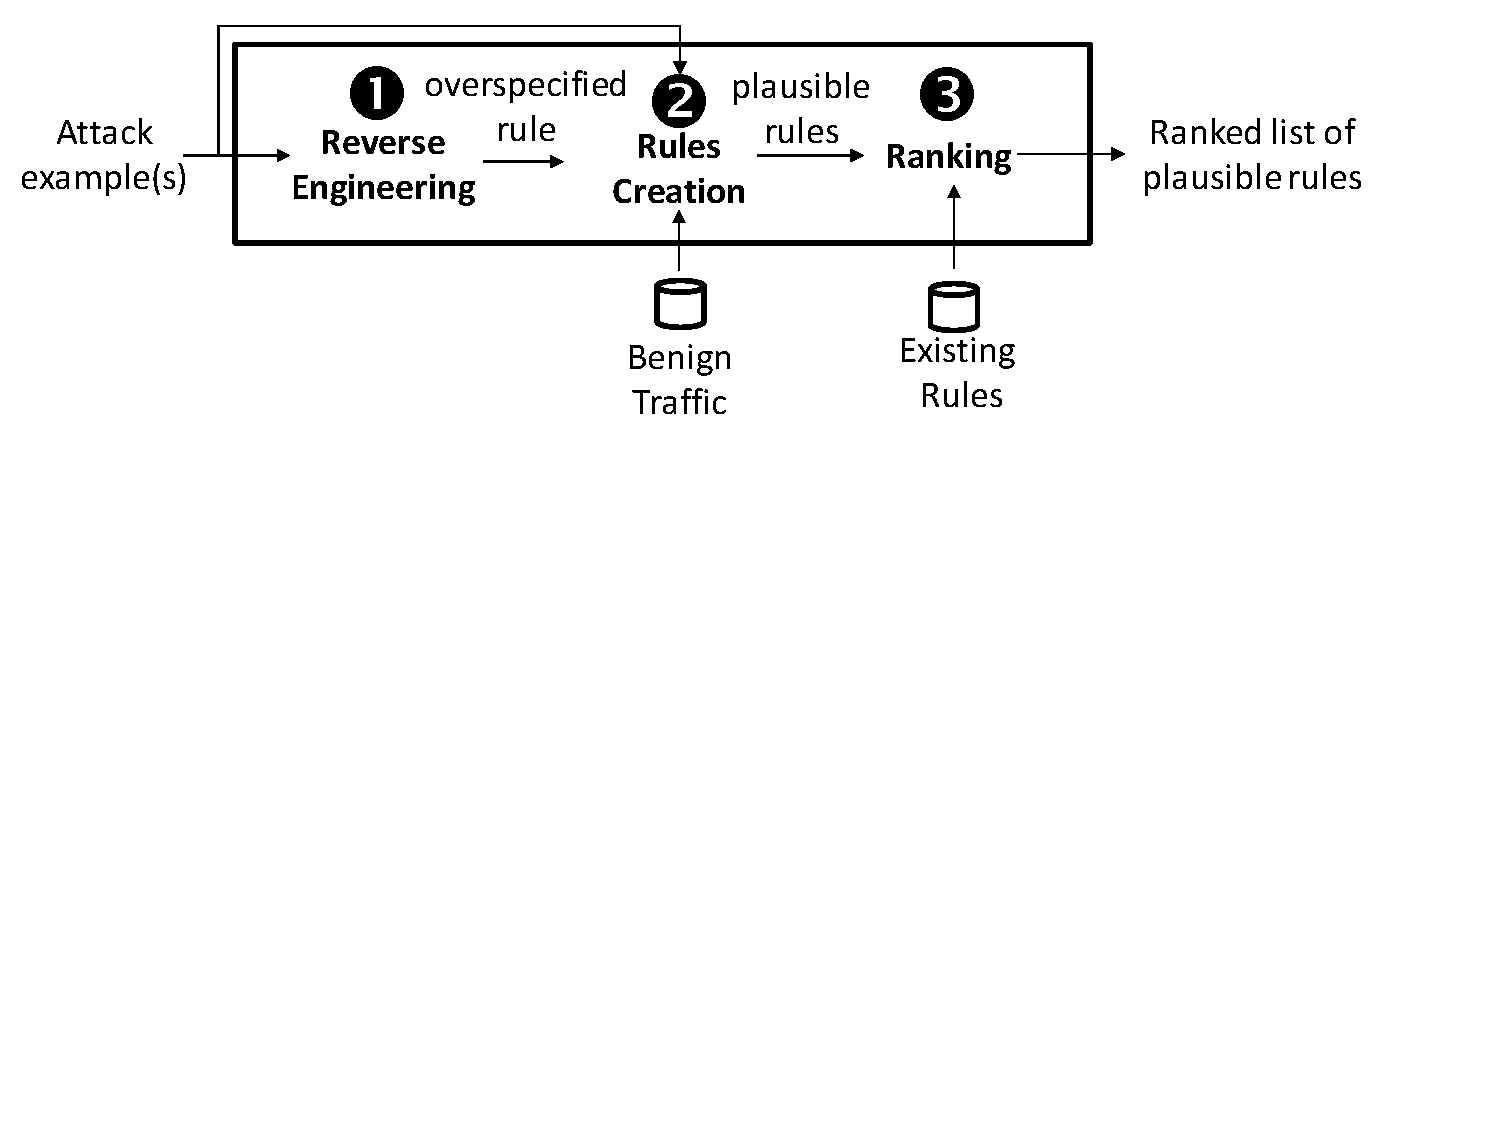
\includegraphics[trim=0 395 50 0,clip,width=0.65\textwidth]{figs/nids-workflow}
  \caption{The \tname\ workflow.}
  \label{fig:overview}
  \vspace{-2ex}
\end{figure*}

\section{Technique}
\label{sec:technique}

\tname{} is a technique to synthesize rules for signature-based
\nids~(\eg{}, Snort~\cite{snort} and Suricata~\cite{suricata}). The
goal is to create rules that capture \emph{only} the
malicious traffic.

\vspace{1ex}
\noindent\textbf{Overview.}~To create rules, \tname\ leverages (1)
benign and malicious network traffic and (2) rules from public
rulesets. \tname\ takes on input malicious and benign traffic and a
set of rules from public rulesets and produces on output a list of
\emph{plausible rules}---\ie{}, rules that isolate the malicious
traffic from the benign traffic---in order of their likelihood to
reflect user's intent. Figure~\ref{fig:overview} shows the workflow of
\tname{} as a pipeline of three components, which appear numbered in
the figure.  Public data sets of benign
traffic~\cite{tcpreplay,stratosphere-normal} and \nids\ rules
exist~\cite{emerging-threats-open}. Consequently, a user of \tname{}
only needs to provide the malicious traffic on input.

\tname\ works as follows. First, it produces a potentially
overspecified rule that captures the malicious traffic, which is
provided on input in the form of pcap files~\cite{pcap}. In this step,
\tname\ detects options directly from the input messages (see
Section~\ref{sec:rules-and-packets}). More precisely, it produces a
rule containing all possible options satisfied by the traffic. Let us
refer to that rule as the \emph{seed rule} and its corresponding set
of options as \emph{seed options}. Note that, as only malicious
traffic is considered in this step, the seed rule is likely
overspecified, \ie{}, it may be more restrictive than the golden rule
(see Section~\ref{sec:suri-metas-coverage}). Consequently, the use of
that rule to capture attacks associated with the input traffic could
lead to false negatives.  Second, \tname\ generates rules that weaken
the constraints associated with the seed options whilst still
capturing the malicious traffic. Given that every option declared in a
rule needs to be satisfied for a rule to capture an attack, any subset
of the set of seed options must capture the malicious traffic by
definition. \tname{} leverages that observation to search for rules
containing a proper subset of options from the seed options. However,
note that that approach alone could result in false positives as it
imposes no limit on to what extent a rule can be relaxed. \tname{}
uses benign traffic for that purpose. More precisely, it uses a
gradient descent-like search to find all plausible rules derived from
the seed rule, obtained in the previous step. Finally, \tname{} uses
several heuristic functions derived from a data set of existing rules
to rank the plausible rules generated in the previous step by their
similarity to existing rules. The rationale is that many plausible
rules can be generated in this step and they have different semantics,
which can differ from user's intent. Similarity is used to approximate
user's intent.


%%  As the generation
%% procedure discards options from the initial rule, the rules \tname{}
%% creates satisfy the property of capturing malicious traffic.



%% The goal of the first
%% component is to produce a rule that captures the negative traffic.
%% First, it initializes the rule with random values. Only options
%% associated with the used protocol are included in the rule
%% representation. Then, \tname\ optimizes the rule options until
%% \suri\ is able to capture the attack associated with the negative
%% traffic.  \tname\ unsuccessfully terminates at this point if it cannot
%% capture the attack. The second component takes as input the rule
%% produced by the first component and tries to minimize that rule. Note
%% that any subset of options would capture the negative traffic---as all
%% options in the rule need to be satisfied for the negative traffic to
%% be captured---but it can also capture positive traffic. This component
%% systematically discards options from the rule encoding until no
%% positive traffic is captured.



\subsection{Step 1: Reverse Engineering}

The first step in the \tname's workflow is Reverse Engineering. The
goal of this step is to extract options from the malicious traffic. A
rule that contains these options, by construction, captures the
malicious traffic. \tname\ uses two strategies to extract options:
1)~field (for any protocol) and 2)~payload (for http only). We
elaborate these strategies in the following.

For the field strategy, \tname{} parses the input messages looking for
options associated with the data in the fields of a network
message. Section~\ref{sec:rules-and-packets} shows the correspondence
between packet fields and some of the rule options from
\suri. Section~\ref{sec:active-recon} shows a concrete example where
the values for options are directly extracted from packet fields. We
obtained the mapping of network fields to options manually, from the
\suri\ documentation.

Unfortunately, the relevant data for the option may be at the message
payload; not the fields. We found empirically that this occurs
frequently in http attacks, which are prevalent. For example,
\Fix{\Luc{53\%}} of the \numrulessuri{} rules from a public data
set~\cite{emerging-threats-open} we analyzed prescribe defenses
against http attacks. Figure~\ref{fig:rule-jboss} shows an example of
a rule that captures traffic containing the string
\CodeIn{"/HtmlAdaptor"} in the payload.  Content options are very
common in http rules---\percRulesWithContent{} of the rules from the
data set mentioned above contain at least one content
option. Figure~\ref{fig:distribution-contents} shows the histogram of
the number of these options per rule for the data set mentioned
above. We limited the number of content options per rule to 10 in the
histogram for space. \MyComment{Rules without \CodeIn{content} options
  are an exception and half of the rules contain at least two
  \CodeIn{content} options.}  Consequently, handling content options
for http is important. The content strategy focuses on extracting such
kinds of options from the payload.

We found, inspecting existing rules, that \CodeIn{content} options
typically refer to sequence of characters in the payload. To find the
values associated with these options, \tname{} splits the payload of
the malicious message in tokens using natural language delimiters,
such as $\backslash$t, $\backslash$n, $\backslash$r, and
spaces. Considering the example from
Section~\ref{sec:content-example}, \tname{} produced a total of 23
tokens, considered content option candidates.

It is worth noting that we found empirically that deciding which
reverse engineering strategy to use based on the protocol of the input
(malicious) messages was effective. We used the payload strategy for
http and the field strategy for the other protocols. For flooding
attacks, \tname\ runs the same approach for each message and
identifies common options across all messages. For that case,
\tname\ reports, in addition, a \CodeIn{threshold} option, as
discussed on Section~\ref{sec:rules-and-packets}.  At the end of the
Reverse Engineering step, \tname\ produces a seed rule that captures
the malicious traffic.

%% \Mar{Nao esta muito claro como isto funciona. Rodamos sempre as duas
%%   estrategias (para obter field options e content options)?
%%   (Precisamos dizer se eh possivel ter regras com os dois tipos de
%%   opcoes). Como isto funciona 1) quando uma ataque tem varias
%%   mensagens (e.g., ping scan) e 2) quando temos varios ataques?}

%% \textbf{Implementation.}~
%% , characterized with pcap files~\cite{pcap}, a popular format
%% to describe network packets.

%% \Fix{
%% A avaliação que fazemos aqui pontua um dado content de acordo com
%% quantas vezes o campo em que ele se encontra eh referenciado nas
%% regras. Por exemplo, vamos supor que o tokenizer produziu a opção
%% content: "/HtmlAdaptor". Essa string pertence ao campo "Request
%% URI:". Esse campo pode ser acessado pelo modificador http\_uri. O
%% tokenizer associa o content a esse modificador.
%% }


\subsection{Step 2: Rule Minimization}
\label{sec:minimization}

\Mar{------------------------------------------- Eu estou aqui}

The rule reported in the first step satisfies the criterion to only
capture positive traffic. Unfortunately, that rule is overconstrained.
The rule can include options that are irrelevant for the input
message. Consequently, the \nids\ may be unable to capture a different
manifestation of the same attack.

%%  Some options added to the rule
%% during the first step are irrelevant for determining the attack and
%% should be removed to obtain more general rules. 

\tname{} leverages public data sets~\cite{tcpreplay} of benign traffic
to guide the search for more general rules, hence addressing the
overffiting issue. To that end, \tname{} \emph{minimizes} the rules
produced in the previous step, preserving the invariant of \emph{only}
capturing the positive malicious traffic. We say that a rule is
minimal if discarding any option results in capturing negative (\ie{},
benign) traffic.  The minimization procedure we propose in this step
builds on the observation that all options from the rule produced in
the previous step are satisifed by the positive traffic. Consequently,
any subset of these options also captures the positive traffic. The
procedure iteratively discards options from the candidate rule until
it detects that the rule is minimal, \ie{}, it finds that no other
option can be removed. The procedure uses negative traffic to guide
the search.



\algdef{SE}[DOWHILE]{Do}{doWhile}{\algorithmicdo}[1]{\algorithmicwhile\ #1}%
\algnewcommand\algorithmicforeach{\textbf{for each}}
\algdef{S}[FOR]{ForEach}[1]{\algorithmicforeach\ #1\ \algorithmicdo}
\algnewcommand\And{\textbf{and} }%
\begin{algorithm}[t!]
  \noindent\hspace{-25ex}
  \textbf{INPUT:} (overconstrained) seed rule $sr$ \\
  \noindent\hspace{-27.5ex} 
  \textbf{OUTPUT:} Set of minimized rules $\mathcal O$\\
%\vspace{-3ex}
\captionof{algorithm}{Minimization algorithm}\label{algo1}
\begin{algorithmic}[1]
  \State $\mathcal R \gets \{\mathit{sr}\}$\Comment{initial population
    of candidate solutions contains only the input
    rule.}\label{line-init}
  \State $\mathcal O \gets \emptyset$
  \Do\label{start-do-while}
      \State $\mathcal R' \gets \emptyset$ \Comment{new iteration. reset.}\label{init-rprime}
      \ForEach {$ro \in \mathcal R $}\Comment{analyze each candidate rule.}\label{start-foreach}
           \For {$i \gets 1$ to $N$}\Comment{mutate each rule $N$ times.}\label{start-for}
               \State $r \gets copy(ro)$      
               \State $j\gets \mathit{rand}(0,\mathit{len}(r))$
               \State $r[j]\gets 0$\Comment{discard option $j$ in $r$}
               \If{$\mathit{isNew(r)} \And \mathit{isPlausible}(r)$} 
                   \State $\mathcal R' \gets \mathcal R' \cup \{r\}$\label{line-progress}
               \EndIf
           \EndFor\label{end-for}
       \EndFor\label{end-foreach}
       \State $\mathcal R \gets \mathcal R'$\Comment{update new generation}
       \State $\mathcal O \gets \mathcal O \cup \mathcal
       R$\Comment{remember all rules}
  \doWhile{$\mathcal R\not= \{\}$}\Comment{repeat until reaching a fixpoint}\label{end-do-while}
\end{algorithmic}
\end{algorithm}

Algorithm~\ref{algo1} shows the pseudocode of the \tname{}
minimization algorithm. The algorithm takes as input the
overconstrained rule produced by the reverse engineering step and
produces a set $\mathcal R$ of minimized rules. Line~\ref{line-init}
initializes the set $\mathcal{R}$ of candidate solutions with the seed
rule $sr$. We encode a rule as a bitvector where each index in the
vector represents one option; the value assigned at a given position
indicates whether or not the option is present in the rule. Each
iteration of the outer loop
(lines~\ref{start-do-while}-\ref{end-do-while}) represents one
generation of the population of individuals produced by the
search. The algorithm terminates when no rule in the current
generation of individuals could be further reduced without violating
the property that a candidate solution should only capture positive
traffic. This means that execution of one iteration has not reached
the statement declared at line~\ref{line-progress}, which adds an
element to the set $\mathcal{R'}$. Consequently, that set will be
empty at the end of one iteration of the outer
loop. Line~\ref{init-rprime} initializes the new generation of
candidate rules. The inner loop
(lines~\ref{start-foreach}--\ref{end-foreach}) iterates through each
candidate rule in $\mathcal R$. Note that these rules have been found
in the previous generation. The algorithm mutates each of these rules
for $N$ times, discarding one option of the rule each time. The call
to $\mathit{isNew}$ checks if $r$ has not been previously generated
through another path whereas the call to $\mathit{isPlausible}$ checks
if the rule only captures positive traffic. Function $\mathit{copy}$
creates a copy of the bitvector of a rule, function $\mathit{len}$
returns the length of the vector, and function $\mathit{rand}$
randomly chooses one index of the vector.

Note that no rules are produced in the last iteration of the
algorithm. Minimal rules are produced in the second-to-last
iteration. In the other iterations, intermediate rules are
produced. Conceptually, the search induces a search tree with the seed
rule $sr$ as the root, minimal rules as child nodes, and intermediate
rules as internal nodes. The edges of the tree denote the ancestor
relation between two rules. Note also that the algorithm reports every
rule in the tree instead of only minimal rules. The reason is that the
correct rule may be non-minimal. In summary, this algorithm reports
many rules that are plausible by using benign traffic to minimize an
overconstrained rule that is focused on the malicious traffic. In the
following step, \tname{} ranks the rules this algorithm reports by
their similarity with previous rules.



\begin{theorem}
  The minimization algorithm computes rules that capture only
  the positive traffic.
\end{theorem}
\begin{proof}
  Every rule created during the search captures the positive traffic
  as every rule contains a proper subset of the option from the
  original rule and all those options are satisfied by the positive
  traffic. By definition of function $\mathit{isPlausible}$, these rules
  also capture \emph{only} the positive traffic. If some negative
  traffic was captured, a rule would not be added to $\mathcal
  R'$.
\end{proof}

\begin{proposition}
  The minimization algorithm may not produce minimal rules.
\end{proposition}

\begin{proof}
The output of the minimization algorithm may contain rules that are
not minimal given the non-determinism of the algorithm. In principle,
it is possible that options that could be discarded are not selected
in the loop from lines~\ref{start-for}--\ref{end-for}. However, we
found empirically that a small value of $N$ suffices to discard those
options from a rule.
\end{proof}

%% Public databases of negative traffic with
%% \Fix{thousands} of messages exist  and can be used to
%% increase the accuracy of the minimization.
%\subsection{Limitations}
%\Fix{...}

\textbf{Implementation details.} We implemented function
\emph{isPlausible} by 1)~updating Suricata to only monitor the rule
that is passed as parameter, 2)~replaying the negative traffic (see
Section~\ref{sec:dataset-benign}), and 3)~reading the Suricata logs to
check if any benign message was captured by the rule. It is worth
noting that the benign traffic is stored in \emph{pcap}
files~\cite{pcap} and Suricata can process those files very
efficiently compared to analyzing network messages directly. Instead
of sending traffic to a machine with a deployed server (\eg{}, web
server) that \suri\ monitors, our setup calls Suricata directly
through an API. Suricata is invoked multiple times in the process of
minimizing the rule.  \textbf{Limitations.} It is worth noting that
although \tname{} is accurate for generating rules that discrimate
positive and negative traffic, the quality of these rules is limited
by the quality of the training data it uses. For the positive traffic,
\tname{} only requires one sample, but can benefit of several
samples. The same applies for the negative traffic. In this case,
however, \tname{} can use public data sets available online.
  


\subsection{Step 3: Ranking}
\label{sec:ranking}

\tname{} uses a composition of heurisitc functions to sort the rules
it produces. Each function uses a different criterion to estimate how
similar a rule, created in the previous step, is to rules from a
public database~\cite{emerging-threats-open} including a total of
\numrulessuri\ rules. We describe in the following each of these
heuristic functions. The codomain of each function ranges in the 0-1
interval. The score of a rule is the average across the values
produced by each function.

%% \Luc{atualmente eh uma
%%   média simples e não ponderada ja q as funções tem o mesmo
%%   peso. conversamos na ultima reuniao sobre testar diferentes pesos
%%   para cada função, mas n sei quão prioritário eh isso comparado as
%%   outras atividades que definimos.} $\sum{f_i}/|f_i|$.

\subsubsection{Size of a rule}
One element that \tname{} uses to measure similarity between a
synthesized and a human-created rule is the size of the synthetic
rule, \ie{}, the number of options it contains. Informally, rules with
popular sizes score high whereas inpopular rules score
low. Figure~\ref{fig:distribution-rule-size} shows the histogram of
rule sizes for our rule data set. The x-axis shows the number of
options included in a rule (up to 10) while the y-axis shows the
number of rules with the corresponding number of options. Note that
there are 11 rules with no options. These rules only use the header to
signal a traffic as malicious. Also note that most rules have 2 to 6
options. \tname{} values rules in that size range higher compared to
other sizes.

%\tname{} uses this information to rank rules.





More precisely, we calculate the contribution of size of a given rule
$r$ with the following formula:

\[\frac{\mathit{rules\_per\_size}[\mathit{len(r)}]}{\mathit{max(rules\_per\_size})}\]

\noindent
, where $\mathit{len(r)}$ denotes the number of options of a rule $r$,
$\mathit{rules\_per\_size}$ encodes distribution of sizes as a
dictionary mapping sizes to number of associated rules, and
$\mathit{max(rules\_per\_size)}$ returns the maximum number of rules
for any dictionary entry. Consequently, the contribution of size is
proportional to its popularity. For example, the contribution of this
heuristic for a rule with three options would be 0.684 (=3,662/5,353)
whereas the contribution of a rule with nine options would be 0.028
(=154/5,353). Note that the measurement is normalized in the 0-1
range.

\subsubsection{Number of content options.} We empirically observed that content options are very
common. \Luc{Se for preciso temos numeros para fundamentar isso
  melhor, sao cerca de 70K contents nas 28K regras do
  data set}\Mar{sim, isto ajuda, porem mais importante eh saber quantas
  (\%) das 28K regras tem contents.} \Luc{92\%} As consequence, we defined a
heuristic function that takes the number of content options into
account. We calculate the contribution of number of content options
with the following formula:

\pgfplotsset{width=6cm,compat=1.8}
\pgfplotsset{every tick label/.append style={font=\tiny}}



\begin{figure*}[t!]
\centering
\begin{subfigure}{.5\textwidth}
  \centering
  \scalebox{1.2}{  
    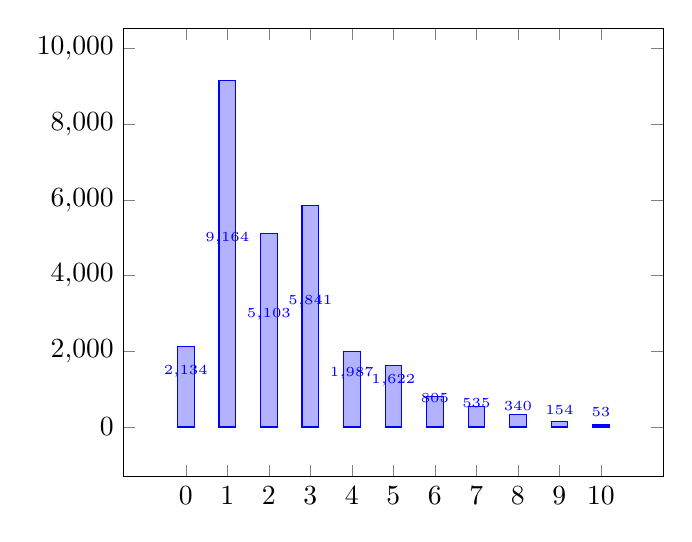
\begin{tikzpicture}
      \begin{axis}[
          bar width=6pt,
          scaled ticks=false,
          tick label style={/pgf/number format/fixed},
          ybar stacked,
          enlargelimits=0.15,
          legend style={at={(0.5,-0.15)},
            anchor=north,legend columns=-1},
          symbolic x coords={0, 1, 2, 3, 4, 5, 6, 7, 8, 9, 10},
          xtick=data,
          nodes near coords,
          every node near coord/.append style={font=\tiny},
          nodes near coords align={vertical},
        ]
        \addplot coordinates {(0,2134) (1,9164) (2,5103) (3,5841) (4,1987) (5,1622) (6,805) (7, 535) (8, 340) (9,154) (10, 53)};
      \end{axis}
    \end{tikzpicture}
  }
  \vspace{-1ex}
  \caption{\label{fig:distribution-contents}Number of content options.}
\end{subfigure}% <---- don't forget this %
%\vspace{1ex}
%\\
\begin{subfigure}{.5\textwidth}
  \centering
  \scalebox{1.2}{
    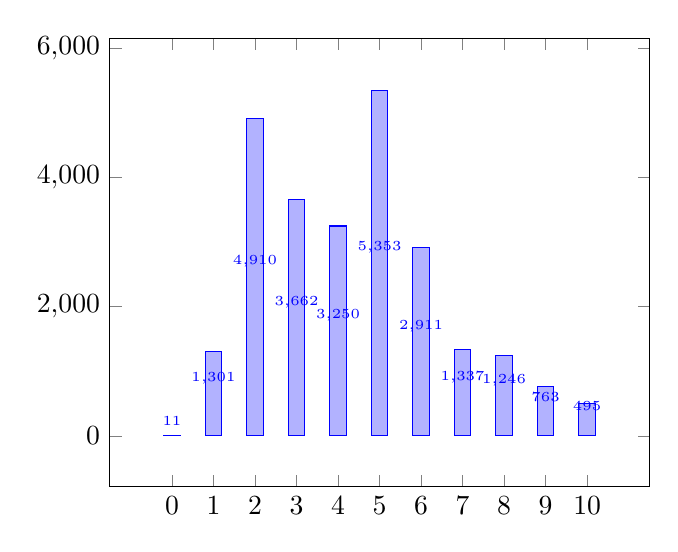
\begin{tikzpicture}
      \begin{axis}[
          bar width=6pt,
          scaled ticks=false,
          tick label style={/pgf/number format/fixed},
          ybar stacked,
          enlargelimits=0.15,
          legend style={at={(0.5,-0.15)},
            anchor=north,legend columns=-1},
          symbolic x coords={0, 1, 2, 3, 4, 5, 6, 7, 8, 9, 10},
          xtick=data,
          nodes near coords,
          every node near coord/.append style={font=\tiny},
          nodes near coords align={vertical},
        ]
        \addplot coordinates {(0,11) (1,1301) (2,4910) (3,3662) (4,3250) (5,5353) (6,2911) (7, 1337) (8, 1246) (9,763) (10, 495)};
      \end{axis}
    \end{tikzpicture}
  }
  \vspace{-1ex}
  \caption{\label{fig:distribution-rule-size}Rule sizes.}
\end{subfigure}%
%\vspace{1ex}
\\
\begin{subfigure}{.5\textwidth}
  \centering
  \scalebox{1.2}{  
    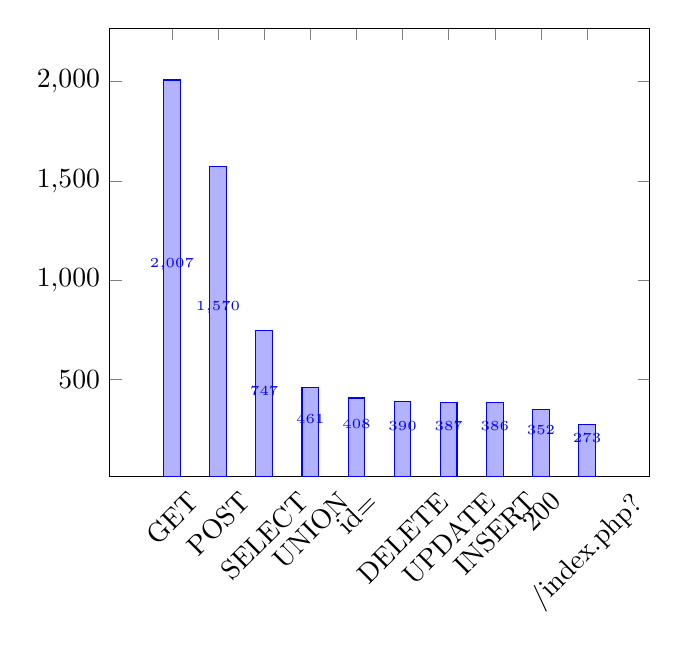
\begin{tikzpicture}
      \begin{axis}[
          bar width=6pt,
          scaled ticks=false,
          tick label style={/pgf/number format/fixed},
          ybar stacked,
          enlargelimits=0.15,
          legend style={at={(0.5,-0.15)},
            anchor=north,legend columns=-1},
          symbolic x coords={GET, POST, SELECT, UNION, id=, DELETE, UPDATE, INSERT, 200, /index.php?},
          xtick=data,
          xticklabel style={rotate=45},          
          nodes near coords,
          every node near coord/.append style={font=\tiny},
          nodes near coords align={vertical},
        ]
        \addplot coordinates {(GET,2007) (POST,1570) (SELECT,747) (UNION,461) (id=,408) (DELETE,390) (UPDATE,387) (INSERT, 386) (200, 352) (/index.php?, 273)};
      \end{axis}
    \end{tikzpicture}
  }
  \vspace{-3ex}  
  \caption{\label{fig:distribution-strings}Strings used as parameters of content options.}
\end{subfigure}%
%\vspace{1ex}
%\\
\begin{subfigure}{.5\textwidth}
  \centering
  \scalebox{1.2}{
    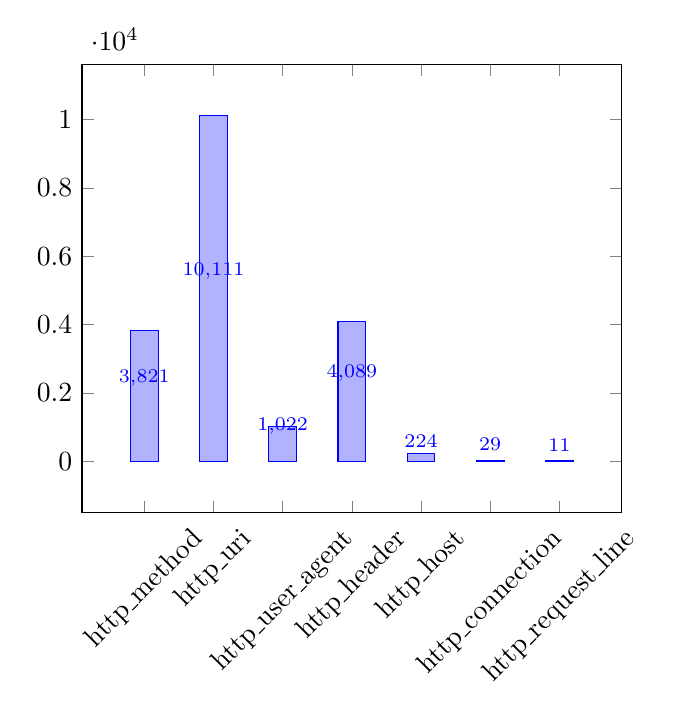
\begin{tikzpicture}
      \begin{axis}[
          ybar stacked,
          enlargelimits=0.15,
          legend style={at={(0.5,-0.15)},
            anchor=north,legend columns=-1},
          %          ylabel={\#rules},
          symbolic x coords={http\_method, http\_uri, http\_user\_agent, http\_header, http\_host, http\_connection, http\_request\_line},
          xtick=data,
          xticklabel style={rotate=45},          
          nodes near coords,
          every node near coord/.append style={font=\scriptsize},        
          nodes near coords align={vertical},
        ]
        \addplot coordinates {(http\_method,3821) (http\_uri,10111) (http\_user\_agent,1022) (http\_header,4089) (http\_host,224) (http\_connection,29) (http\_request\_line,11)};
      \end{axis}
    \end{tikzpicture}
  }
  \vspace{-1ex}
  \caption{\label{fig:distribution-content_modifiers}Content modifiers
    frequency.}
\end{subfigure}%
\vspace{-1ex}
  \caption{Distribution of features.}
\end{figure*}


\[\frac{\mathit{rules\_per\_number\_of\_contents[len(r)]}}{\mathit{max(rules\_per\_number\_of\_contents)}}\]

\noindent
Note that the only difference of this formula compared to the formula
to compute contribution of size is the distribution used, which is
given by the term $\mathit{rules\_per\_number\_of\_contents}$ denoting
a dictionary of number of content options to number of rules that
contain that number of content options.

\subsubsection{Content rarity.} 
This heuristic weighs higher rules that use popular strings in content
options. For a given rule \tname{} takes the arithmetic mean of the
popularity scores of each string used in contents in that rule. More
precisely, we calculate the contribution of content rarity with the
following formula:

\[\frac{\sum_{i=1}^{N}\frac{\mathit{content\_frequency[content_i]}}{\mathit{max(content\_frequency)}}}{N}\]

\noindent
, where the term $\mathit{content_i}$ denotes the $i$-th xcontent in a
given rule, the term $\mathit{content\_frequency[\mathit{content_i}]}$
denotes the frequency of the string used in the $i$-th content, the
term $\mathit{max(content\_frequency)}$ denotes the maximum frequency
observed across all strings appearing as content parameters, and $N$
is the number of content options in a given
rule. Figure~\ref{fig:distribution-strings} shows the distribution of
the ten most popular strings in our rule data set. To illustrate this
function, let us consider a rule with two content options, using the
strings ``GET'' and ``ID'', respectively. The contribution of that
rule for the computation of similarity score would be 0.601
(=(1+.203)/2).



\subsubsection{Frequency of content modifiers.} As previously
mentioned, \percRulesWithContent\ (=26K/\numrulessuri) of Suricata
rules involve content options. Furthermore, of the 26K rules that use
content options, 13K use HTTP modifiers\Mar{@Lucas, pode dar o numero
  desconsiderando HTTP? Esta parte eh generica.}. \Luc{Posso, mas nessa função nós consideramos apenas os modificadores http.} Content modifiers
serve to indicate what part of a network packet the string mentioned
in the content option should appear. For example, the modifier
\CodeIn{http\_header} in the option \CodeIn{content: ``keep-alive'';
  http\_header} states the requirement that the string ``keep-alive''
be present in the header of the message. (A keep-alive connection
attribute indicates that a single TCP connection should remain open
for multiple HTTP requests/responses.)
Figure~\ref{fig:http-header-example} illustrates possible content
options used to match against certain strings that appear in an HTTP
message. A check (resp., cross) mark indicates a match (resp.,
unmatch).

\begin{figure}[t!]
\centering
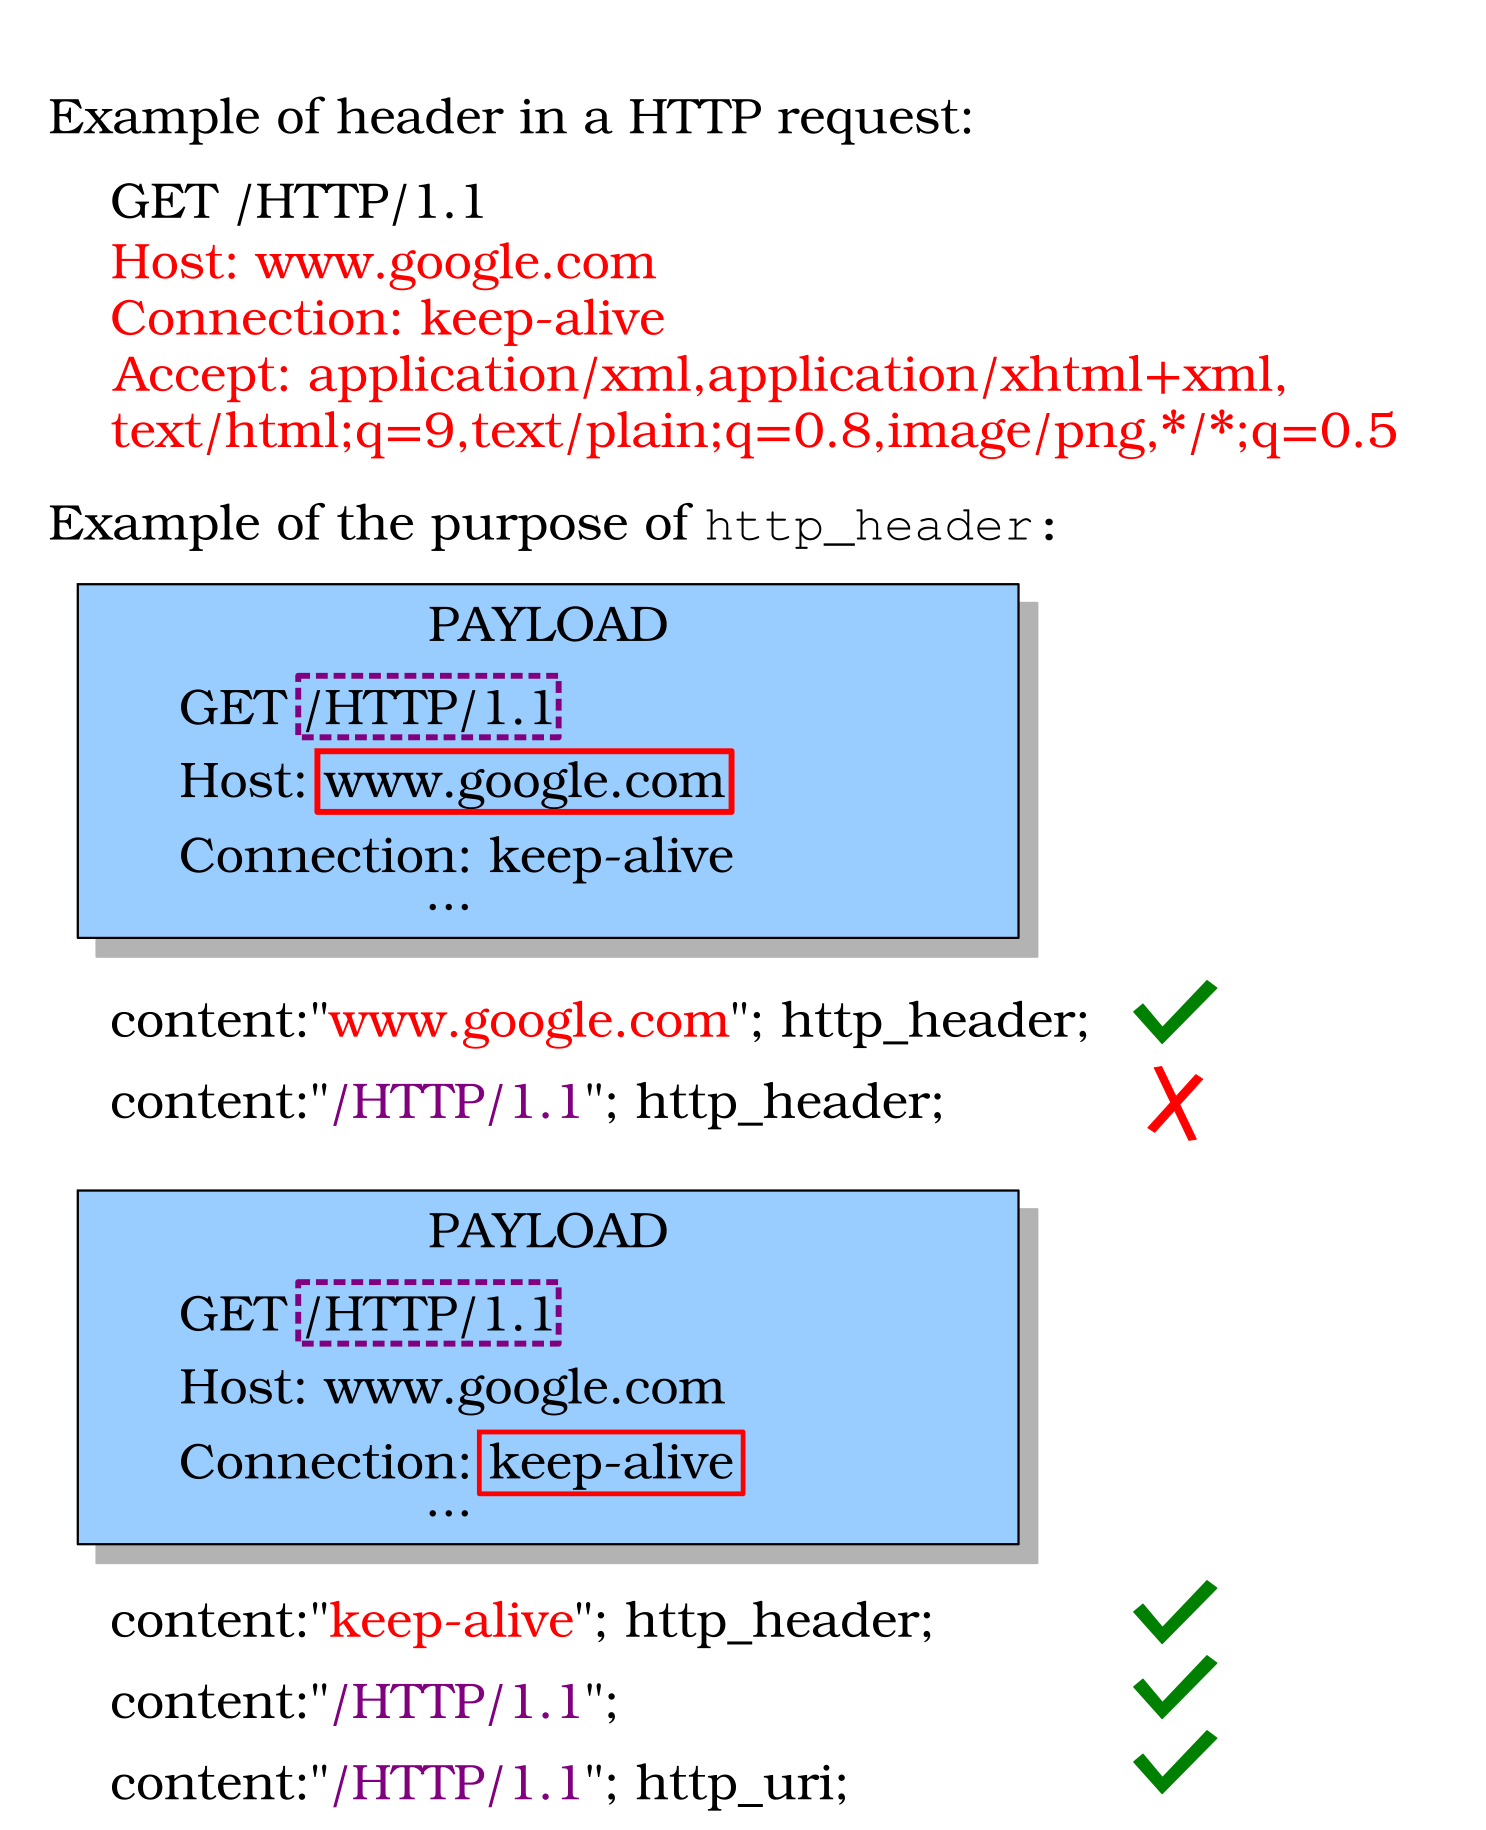
\includegraphics[scale=0.5]{figs/http_header-example.png}
\caption{\CodeIn{http\_header} example.}
\label{fig:http-header-example}
\end{figure}

%% we observed---by analyzing
%% the data set of existing rules (see
%% Section~\ref{sec:data set-benign})---that these rules often indicate
%% what part of the message the content string should be checked
%% against. For example,
%% For example, the
%% creator of the rule may want to indicate that a specific string be
%% present in the header of an HTTP request message. Content
%% \emph{modifiers} serve this purpose.
%% Suricata supports content modifiers for tcp and http. \Luc{Eh possivel utilizar os modificadores em qualquer protocolo. Nós consideramos apenas tcp e http pois são os protocolos que possuem payloads legiveis, assim conseguimos saber melhor como tokenizar o conteudo. O payload de pacotes de outros protocolos, em geral, são um conjunto de bytes sem significado para nós. Existem diversos outros modificadores q não estamos considerando e q tambem permitem procurar numa determinada posição para os casos em q o conteudo do pacote n eh legivel, não citei pq não suportamos isso. Se necessário posso explicar.} Given that
%% content options often use modifiers\Mar{assumindo que eh
%%   verdade. confirmar estat. solicitada acima...},

\tname{} leverages the fact that these modifiers are commonly used to
define rules as to better rank the rules it synthesizes. More
precisely, it builds on the observation that strings acessible in
positions associated with content modifiers (\eg{}, GET, Host,
Connection) are more likely to produce useful rules. \tname\ uses the
frequency of content modifiers to discriminate rules that are more or
less likely to reflect actual rules. For example, historical data
indicates that content options that use the \CodeIn{http\_connection}
modifier are much less likely than content options that use the
modifier
\CodeIn{http\_uri}. Figure~\ref{fig:distribution-content_modifiers}
shows the histogram of content modifiers for http. Although content
modifiers are applicable to rules of any protocol supported by
Suricata, currently, \tname\ only supports tcp and http. These are the
protocols involving ~80\% of the rules from our data set.

%% and
%% (2) the payload of messages of different protocols are not as
%% segmented as the case of tcp and http. Consequently, rule writers do
%% not refer to specific parts of the payload as often as the task o and
%% more challenging for

Similarly to the the previous heuristic functions, this function uses
the frequency of content modifiers to calibrate the score of each
rule. More precisely, we compute this function with the following
formula:

\[\frac{\sum_{i=1}^{N}g(i)}{N},~g(i)=\frac{\sum_{j=1}^{M_i}\frac{\mathit{modifier\_frequency[modifier_{ij}}]}{\mathit{max(modifier\_frequency)}}}{M_i}\]

\noindent
, where $N$ is the number of contents options, $g(i)$ is the
contribution of content option $i$ to the score,
$\mathit{modifier\_frequency[modifier_{ij}}]$ denotes the popularity
of a modifier $j$ to content option $i$,
$\mathit{max(modifier\_frequency)}$ refers to the modifier with
maximum popularity (for normalization), and $M_i$ is the number of
content modifiers that could access the string associated with content
$i$.


%% \Mar{Qual o rationale para considerar as varias
%%   alternativas de acesso ao inves de apenas a alternativa que eh mencionada?}0
%%   \Luc{Vc está supondo que as regras que geramos incluem os modificadores e que deveriamos pontuar somente de acordo com os que estão presentes? Não eh o caso. A ideia aqui basicamente eh: se um certo content do payload está numa posição q eh muito verificada nas regras, possivelmente esse content eh mais relevante do q outro q está numa posição q raramente eh verificada. Para avaliar isso nós só precisamos saber quantas vezes os modificadores que acessam essas posições aparecem no data set.}
%%   \Luc{Uma coisa que pensei agora foi de considerar apenas o modificador mais comum entre aqueles que acessam a posição de um content. Como a pontuação de um content eh dado pela media das ocorrencias dos modificadores que conseguem acessá-lo, se houver um modificador muito comum e varios modificadores raros a pontuação dada será baixa.}
                                                                             
%% \Luc{$M_i$ eh o numero de modificadores que podem referenciar a posição em q se encontra o $content_i$}\Mar{isto eh confuso. vc. esta dizendo que
%%   o mesmo content pode ter mais de um modificador? ou a string poderia
%%   ser acessada por mais de um modificador. se for este o caso,
%%   sinceramente, achei isto bem confuso. afinal, a regra jah indica
%%   qual o modificador foi escolhido para acessar a string.}.\Luc{Cada content em uma regra só pode possuir um modificador para indicar a posição onde ele deve ser procurado. Entretanto sim, uma "string poderia
%%   ser acessada por mais de um modificador", foi o caso daquele exemplo com o http\_header.} \Luc{M eh
%%   o numero de modificadores associados a cada content. Temos
%%   content[1], content[2], ..., content[N]. Cada um desses contents tem
%%   modificadores associados content[i][1], content[i][2], ...,
%%   content[i][M].}\Mar{Lucas, e se nao houver modificador algum em um
%%   content. a frequencia seria 0, correto?} \Luc{Sim}


%\Mar{what about ``none'' (no modifier)?}}
%  \Luc{Uma regra pode sim ter contents sem modificadores, mas isso n
    %% vem ao caso aqui. Nessa heuristica toda string do payload vai ter
    %% associada a ela os modificadores q podem acessar a sua
    %% posição. Portanto, não vai existir o caso de não haver
    %% modificador. Atenção: isso não quer dizer q as regras q geramos
%% incluem os modificadores, elas n incluem.
%\Luc{Inclui esse modificador pq ele tambem pode acessar o campo Request URI. Isso eh um problema? O http\_uri eh o modificador mais comum, mas o fato de haver o modificador http\_request\_line que tambem accessa a mesma posição faz com que o fitness maximo seja 0.5, pois a ocorrencia de http\_request\_line eh irrelevante no calculo.}
    
Consider a rule containing the option \CodeIn{content:
  ``/HtmlAdaptor''}. The contribution of this option to the score of
the rule that uses it would be $0.5$
(=$\frac{10,111+11}{10,111*2}$). The value of $M_i$ for this case is 2
as the field of the HTTP message \CodeIn{Request URI}---holding the
string ``/HtmlAdaptor''---can be accessed through the modifiers
\CodeIn{http\_uri} and \CodeIn{http\_request\_line}. The relatively
high heuristic value given to this option suggests it is a plausible
option to be used in rules---the string used in the content option
(``/HtmlAdaptor'') is stored in a specific field of the HTTP message
(\CodeIn{Request URI}) and can be accessed by two content modifiers,
namely (\CodeIn{http\_uri} and \CodeIn{http\_request\_line}). For the
option \CodeIn{content: ``keep-alive''}, either the modifier
\CodeIn{http\_header} or the modifier \CodeIn{http\_connection} could
be used to locate the string ``keep-alive'' stored in the field
\CodeIn{Connection} (see Figurgure~\ref{fig:http-header-example}). Consequently, for this
case, the contribution of modifiers to this content option would be
$0.2$ (=$\frac{4089+29}{10111*2}$). Assuming that both options are
used in a rule, the aggregated contribution of this heuristic function
would be 0.35 (=(0.2+0.5)/2).

\Gui{Fizemos um teste para encontrar melhores pesos para cada ataque. Calculamos o fitness de cada regra atribuindo diferentes pesos para cada função heurística. Os valores atribuídos foram 0, 0.25, 0.5, 0.75 e 1. Depois de calculado, ordenamos todas as listas criadas e pegamos a posição da Golden Rule. As melhores combinações de pesos (que conseguiram melhor posição da golden rule) estão na tabela 4, onde na coluna "Weights", há quatro números separados por vírgula, cada um deles representando o peso de uma função (na ordem que é representado no paper. O total de regras criadas é igual ao da Tabela 3.}

%% \section{Modificadores}É possivel deixar que uma regra verifique todo o payload do pacote em busca de um match com um content ou especificar partes do payload onde esse content deve ser procurado. Essa definição é feita utilizando os chamados modificadores de content, eles adicionam mais detalhes/informações sobre a detecção de um determinado content. Os modificadores que estamos considerando são validos apenas para regras dos protocolos tcp e http.

%% Exemplo do payload "cru" de um pacote http:\\
%% Aqui, todas as informações do pacote estão juntas.

%% \begin{figure}[h!]
%%   \lstinputlisting[language=C,numbers=none,keywords={content}]{http-example.payload}
%% \end{figure}

%% O mesmo payload interpretado pelo Wireshark:\\
%% Aqui, o wireshark interpreta as informações dos pacotes e as divide para melhor visualização e entendimento.

%% \begin{figure}[H]
%%   \lstinputlisting[language=C,numbers=none,keywords={content}]{http-example-wireshark.payload}
%% \end{figure}

%% O que o suricata faz eh identificar os campos e seus valores e com isso permite que as regras façam referencia direta a eles. Por exemplo, na figura do payload "cru" não conseguimos identificar facilmente oq eh o "Request URI Path:", já na segunda figura isso está explícito.

%% Eu disse que o "GET" estava associado tambem ao http\_header, mas não está, me enganei. Mas sim, pode haver interseção entre os campos que dois ou mais modificadores referenciam. O seguinte trecho do payload é acessado pelo modificador http\_header:

%% \begin{figure}[H]
%%   \lstinputlisting[language=C,numbers=none,keywords={content}]{http-header.payload}
%% \end{figure}

%% Entretando, tambem existem os modificadores http\_host,
%% http\_accept\_enc, http\_connection e http\_accept que permitem
%% acessar diretamente cada uma das linhas acima.

%% \Mar{Lucas, use uma regra concreta com a regra da Secao 3.3 (assumindo
%% que vai mante-la) e mostre como eh feito o calculo da regra desta
%% funcao heuristica para regra inteira.}\\
%% \Luc{-------------}



%% A avaliação que fazemos aqui pontua um dado content de acordo com quantas vezes o campo em que ele se encontra eh referenciado nas regras. Por exemplo, vamos supor que o tokenizer produziu a opção content: "/HtmlAdaptor". Essa string pertence ao campo "Request URI:". Esse campo pode ser acessado pelo modificador http\_uri. O tokenizer associa o content a esse modificador. 
%% Posteriormente, esse content vai receber uma pontuação
%% correspondente a popularidade desse modificador:\\


%% A multiplicação por 1 no denominador eh referente a quantidade de
%% modificadores que estão associadas a esse content.\Luc{O correto eh ser dividido pela quantidade de modificadores. Atualizei a formula para tentar representar isso. Considere que no exemplo acima o content pudesse ser acessado por mais de um modificador. A pontuação dele então seria $\frac{10,111+x}{10,111*1}$ > 1. Para manter a pontuação entre 0-1, o certo nesse caso seria fazer $\frac{10,111+x}{10,111*2}$}\Mar{nao foi isto
%%   que vc. disse acima, Lucas. foi dito que N (=2) era o numero de
%%   contents e o exemplo acima tem apenas 1 content.}  

%% Content options are
%% associated with specific packets fields\Mar{or modifiers?}.\Mar{why
%%   GET is associated with http\_method and http\_header?}\Mar{are all
%%   content associated with one or many fields or positions in a packet?
%%   can you give examples other than GET to explain this? if yes,
%%   shouldn't this be discussed before? Maybe Section 2.3?}\Mar{Also, it
%%   is important to justify (to explain rationale)---how is it different
%%   from counting rarity?}


%% Esse componente pontua um content de acordo com o campo ao qual ele pertence no pacote. Contents que pertencem a campos mais comuns (campos que são mais referenciados nas regras) recebem maior pontuação.
%% Modificadores diferentes podem acessar campos iguais em um pacote. Por
%% exemplo os modificadores http\_method e http\_header, o http\_method
%% acessa apenas o metodo do pacote http, mas o http\_header acessa todo
%% o cabeçalho (incluindo o proprio metodo). Com isso, a string "GET"
%% receberia a pontuação correspondente a esses dois modificadores.

\begin{table*}[t!]
  \small
  \caption{\label{table:attacks}List of attacks.}
  \centering
  \begin{tabular}{llllp{10cm}}
    \toprule
    \multicolumn{1}{c}{Name} &
    \multicolumn{1}{c}{Source} &
    \multicolumn{1}{c}{Type} &
    \multicolumn{1}{c}{Protocol} &
    \multicolumn{1}{c}{Groud Truth (relevant/checked options)} \\
    \midrule     
    Ping Scan & NMAP & AREC & ICMP & \textbf{dsize}:0; \textbf{itype}:8; \\
    SYN Flood & hping3 & DoS & TCP & \textbf{flags}: S,12; \textbf{threshold}: type both, track by\_dst, count 5000, seconds 5;\\

    JBoss JMX\MyComment{ Console Beanshell Exploit} & Nikto2 & RCE & HTTP \MyComment{& Remote Code Execution} & \textbf{content}:"/HtmlAdaptor"; nocase; http\_uri; \textbf{content}:"action=inspect"; nocase; http\_uri; \textbf{content}:"bean"; nocase; http\_uri; \textbf{content}:"name="; http\_uri; \\
    WeBid \MyComment{Local File Inclusion} & RFI & HTTP & \Fix{LFI} & \textbf{content}:"GET "; depth:4; \textbf{content}:"/cron.php?"; http\_uri; nocase; \textbf{content}:"include\_path="; http\_uri; nocase; \textbf{content}:"../"; \\
    ColdFusion \MyComment{PESC} & Nikto2 & PESC & HTTP \MyComment{& Privilege Escalation} & \textbf{content}:"GET"; http\_method; nocase; \textbf{content}:"/CFIDE/administrator"; http\_uri; nocase; \\
    .htaccess access\MyComment{attempted-recon} & Nikto2 & AREC & HTTP \MyComment{& Adicionar} & \textbf{content}:".htaccess"; nocase; http\_uri; \\
    .idq access\MyComment{EXPLOIT ISAPI} & Nikto2 & RCE & HTTP \MyComment{& Adicionar} & \textbf{content}:".idq"; nocase; http\_uri; \\
    iisadmin access\MyComment{web-application-attack} & Nikto2 & RCE & HTTP \MyComment{& Adicionar} & \textbf{content}:"/iisadmin"; nocase; http\_uri; \\
    /system32/ in URI\MyComment{Possible Protected Directory Access Attempt} & Nikto2 & AREC & HTTP \MyComment{& Adicionar} & \textbf{content}:"/system32/"; nocase; http\_uri; \\
    Script tag in URI\MyComment{Possible Cross Site Scripting Attempt} & Nikto2 & RCE & HTTP \MyComment{& Adicionar} & \textbf{content}:"</script>"; nocase; http\_uri; \\
    Apache Struts 2 & \Fix{Source} & \Fix{RCE} & HTTP & \textbf{content}:"POST"; http\_method; \textbf{content}:"java.lang.ProcessBuilder"; nocase; http\_client\_body; fast\_pattern; \textbf{content}:"/struts2-rest-showcase/orders/3"; http\_uri; \\
    WordPress Login & \Fix{Source} & Policy Violation & HTTP & \textbf{content}:"log="; http\_client\_body; \textbf{content}:"\&pwd="; http\_client\_body; \textbf{content}:"\&wp-submit="; http\_client\_body; \\
    \bottomrule
  \end{tabular}
\end{table*}


\section{Evaluation}

This section reports on the evaluation of \tname{}.


\newcommand{\textRQone}{How well \tname\ ranks the golden rule?}
\vspace{0.2cm}
\begin{itemize}[leftmargin=*,label={}]
\item{\textbf{RQ1.}} \textRQone
\end{itemize}

\noindent
\textbf{Rationale.}~The golden rule is a trusted human-written
\nids\ rule that we obtained from credible sources. \tname\ generates
several rules that satisfy the invariant to only capture the malicious
traffic, but the amount of data we used to evaluate that property,
albeit large, is limited. Assessing the quality of each rule
\tname\ produces (\ie{}, fitness to the attack) requires domain
knowledge and much effort. The position of the golden rule at the
ranking produced by \tname\ is a proxy measure to the effort of a
system administrator in finding the rule that fits the purpose.


\newcommand{\textRQtwo}{How important are the heuristic functions
  to \tname's performance?}
\vspace{0.2cm}
\begin{itemize}[leftmargin=*,label={}]
\item{\textbf{RQ2.}} \textRQtwo\
\end{itemize}

\noindent
\textbf{Rationale.}~We proposed a variety of heuristic functions to
rank the plausible rules that \tname\ created during minimization (as
per step 2 in the workflow). Recall that these functions are based on
the data from a public ruleset~\cite{emerging-threats-open} (see
Section~\ref{sec:ranking}). It is therefore important to understand
the extent to which each function contributes to the overall
performance of the technique.

\newcommand{\textRQthree}{How important are the benign and
  malicious traffic to \tname's performance?}
\vspace{0.2cm}
\begin{itemize}[leftmargin=*,label={}]
\item{\textbf{RQ3.}} \textRQthree\
\end{itemize}

\noindent
\textbf{Rationale.}~\tname\ uses both positive and negative examples
to generate rules. This question investigates how sensible the
technique is to the selection of these inputs.
\noindent
\vspace{1ex}

The following sections describe the objects we used to evaluate the
technique (Section~\ref{sec:dataset-benign}), answer the posed
research questions (sections~\ref{sec:answer-rqone},
and~\ref{sec:answer-rqtwo}, and~\ref{sec:answer-rqthree}), and
discuss threats to the validity of the
experiments~(Section~\ref{sec:threats}).


\setlength{\tabcolsep}{3pt}
\begin{table}[h!]
  \small
  \caption{\label{table:results}Results.}
  \vspace{-2ex}
  \centering
  \begin{tabular}{lrrrr}
    \toprule
    \multicolumn{1}{c}{\multirow{2}{*}{Name}} &
    \multicolumn{1}{c}{\multirow{2}{*}{\# Vars.}} &
    \#~Option Cand. &
    \#~Plausible Rules &    
    \multicolumn{1}{c}{Rank} \\

     &
    \multicolumn{1}{c}{} &
    \multicolumn{1}{c}{(step 1)} &
    \multicolumn{1}{c}{(step 2)} &    
    \multicolumn{1}{c}{(step 3)} \\

    \midrule
    Ping Scan & 5 & 5 & 2 & - \\
    SYN Flood & 3 & 2 & 2 & - \\
    JBoss JMX & 4 & 23 & 228 & \Fix{23} \\
    WeBid & 1 & 23 & - & -\\    
    ColdFusion & 6 & 19 & 34 & \Fix{5}\\
    .htaccess access & 4 & 17 & 984 & \Fix{2}\\
    .idq access & 13 & 19 & 511 & \Fix{2} \\
    iisadmin access & 3 & 17 & \Fix{861} & \Fix{1} \\
    /system32/ in URI & 3 & 20 & 1,913 & \Fix{2} \\
    Script tag in URI & 22 & 22 & 786 & - \\
    Apache Struts 2 & - & - & - & - \\
    Wordpress Login & - & - & - & - \\
    \bottomrule
  \end{tabular}
\end{table}


%%\begin{table}[h!]
%%  \small
%%  \caption{\label{table:weight}Weight Combinations.}
%%  \centering
%%  \begin{tabular}{lrrp{15cm}}
%%    \toprule
%%    \multicolumn{1}{c}{Name} &
%%    \multicolumn{1}{c}{Weights} &
%%    \multicolumn{1}{c}{Rank} \\
%%    \midrule
%%    Ping Scan & - & - \\
%%    SYN Flood & - & - \\
%%    JBoss JMX & 1,0,1,1 & 107 \\
%%    WeBid & - & - \\    
%%    ColdFusion & 0,1,1,1 & 7 \\
%%    .htaccess access & 0,1,1,1 & 11 \\
%%    .idq access & 0,1,1,1 & 7 \\
%%    iisadmin access & 0,1,1,1 & 2 \\
%%    /system32/ in URI & 0,1,1,1 & 11 \\
%%    Script tag in URI & 0,1,1,1 & 9 \\
%%    \bottomrule
%%  \end{tabular}
%%\end{table}
%%

\subsection{Objects of Analysis}
\label{sec:dataset-benign}
\label{attack-reproduction}

This section describes the objects used in \tname{}'s evaluation.

\vspace{1ex}
\subsubsection{Attacks.}~Table~\ref{table:attacks} shows the selection
of attacks considered in our evaluation.  Column ``Name'' shows the
name of the attack, column ``Source'' shows the source where we
obtained data to reproduce the attack (see
Section~\ref{subsec:malicious-traffic}), column ``Type'' shows the
kind of attack, column ``Protocol'' shows the name of the protocol
explored in the attack, and column ``Ground Truth'' shows the rule
options to capture the attack. The rationale for the selection were
(1) to cover attacks with different characteristics, (2) to cover
attacks of various protocols, and (3) to explore different features of
\tname. As for (1), the selection includes attacks of the following
types: Denial-of-Service (DoS), Active Reconnaissance (AREC),
Privilege escalation (PESC), Remote Code Execution (RCE), \Luc{Local 
File Inclusion (LFI) and Policy Violation (PV)}. Note that the 
distribution of attacks is not uniform across protocols as these 
distributions are not uniform in practice---http attacks are prevalent. 


%% It is important to note that this setup is \emph{not}
%% necessary if \emph{pcap} files for the attack already exist. We
%% proceeded as follows to obtain pcap files for the the attacks we
%% analyzed: we 1)~instantiated the script (\eg{}, defined the IP of the
%% web server), 2)~executed the script, 3)~and monitored the traffic with
%% the Wireshark network monitor. The
%% Wireshark tool records the traffic and reports pcap files on output
%% for replaying it.



\subsubsection{\label{subsec:malicious-traffic}Malicious traffic.}~Recall that \tname\ takes
pcap files on input. As explained on Section~\ref{sec:minimization},
these files abstract network messages~\cite{pcap} and can be used to
avoid network traffic during rule synthesis. For some of the attacks
listed on Table~\ref{table:attacks}, we obtained pcap files directly
from trusted security websites (\eg{},
NetReseC~\cite{pcap-attacks}\Fix{confirm}).\Mar{reminder: we still
  don't have any example of attack listed on Table~\ref{table:attacks}
  whose pcap file was obtained from those websites.} \Luc{Ataques Apache 
  e WordPress. @Guilherme adicionar fontes} In addition to
these sources, we used the Nikto2~\cite{nikto} open source security
tool as follows to obtain pcap files for (non-flooding) http and tcp
attacks. We configured an http server (Apache2) and ran Nikto2 to
attack that server. Simultenously, we ran
WireShark~\cite{wireshark-net-monitor} to record the network traffic
and Suricata to analyze the traffic. We configured \suri\ with all
rules from the ``Emerging Threats Open
Ruleset''~\cite{emerging-threats-open} and configured Nikto2 with
default parameters, which makes it replay all recorded attacks. After
execution, we inspected the \suri\ log to identify which rules have
been activated and which packets were involved on each
activation. With the packet numbers, it is possible to recover the
corresponding pcap files, using Wireshark, as to ran \tname{} on
them. It is worth noting that some rules are triggered multiple times,
indicating that Nikto2 expresses multiple variants of the same
attack. RQ3 evaluates the importance of these variants to \tname{}'s
performance. We used similar methodology to obtain pcap files using
other security testing tools. We used NMAP~\cite{netmap} to reproduce
the Ping Scan attack (see Section~\ref{sec:active-recon}) and
hping3~\cite{hping3} to reproduce the SYN Flood attack (see
Section~\ref{sec:dos}).

%% \Mar{@Lucas, diga exatamente como vc. obtem as variacoes. isto eh que
%%   eh importante para a proxima sentenca.}.  \Luc{Eh feito da mesma
%%   forma q foi descrita acima. Quando um ataque produz varios pacotes
%%   que geram alertas, nos criamos um pcap com um dos pacotes e
%%   utilizamos ele como para gerar a regra maxima inicial.  Os outros
%%   pacotes sao salvos em um outro pcap e sao utilizados para calcular o
%%   recall.}


%% \Mar{what about the variants? where do
%%   they come from? this is confusing as the narrative above suggests
%%   the attack is hardcoded in the tool.}\Luc{O trafego de um ataque
%%   normalmente possui varios pacotes, entre esses varios pacotes alguns
%%   deles possuem um padrao. As regras sao criadas descrevendo esse
%%   padrao, com isso um unico ataque pode disparar varios alertas.
  
%%   Porem, existem ataques q so produzem um alerta, ou seja, a regra criada 
%%   so detecta um dos pacotes do trafego. Nesses casos, procuramos na internet 
%%   datasets (arquivos pcap) que contivessem mais pacotes desses ataques.
%%   Fizemos isso tambem para ataques q nos ja tinhamos variacoes, pois
%%   (teoricamente) quanto mais variacoes, melhor. Existem alguns sites onde 
%%   eh possivel encontrar pcaps com o trafego de alguns ataques, n consegui
%%   adicionar nas referencias: 
%%   https://www.netresec.com/?page=PcapFiles
%% }

%% According to the TcpReplay web
%% site ``This capture is much larger and has a smaller average packet
%% size than the previous capture (smallFlows.pcap). It also has many
%% more flows and different applications.''

\subsubsection{Benign traffic.}~Public data sets of bening traffic
exist; they are important to evaluate the rate of false positives of
security tools. We used two popular public sources. The Bigflows.pcap
data set is part of the TcpReplay~\cite{tcpreplay} open source
project. It includes real network traffic of a busy private network
access point to the Internet. In addition to the Bigflows.pcap data
set, we also used data sets\Mar{more than one?}  made available by
Stratosphere Lab~\cite{stratosphere-normal}\Mar{is there a description
  of the traffic? as the description for
  Bigflows.pcap?}. \Luc{@Guilherme ...}

\subsubsection{Ground Truth.}To evaluate \tname\ objectively we need
to compare the rules it generates with \emph{trusted rules}. We used
the ``Emerging Threats Open Ruleset''~\cite{emerging-threats-open} for
that. After finding the attack and corresponding rule using the
procedure described in Section~\ref{subsec:malicious-traffic}, we
reproduced the attack and confirmed that the rule captures the
attack. Column ``Ground Truth'' from Table~\ref{table:attacks} only
shows the essential relevant options. Documentation options (\eg{},
``msg'') are discared.

%% Note from Figure~\ref{fig:overview} that the positive traffic is an
%% input to the technique. The negative non-malicious traffic, however,
%% is not.


%subsection{Methodology}


%% \Gui{
%% O procedimento que já tínhamos representa a etapa de treinamento. Toda aquela parte que foi explicada na apresentação para os outros professores e descrito no paper. Descreverei novamente pra confirmar, e também foi adicionado uma pequena etapa.

%% TREINAMENTO

%% ->Syrius recebe como input um pcap contendo o ataque (no caso de ataques com content, usamos ataques do Nikto), um pcap benígno (usamos o bigflows.pcap) e um pcap contendo as variações de ataque (isso pode ser otimizado unificando com o pcap de ataque, mas por agora está assim)
%% ->É gerado a regra máxima através do tokenizer e engenharia reversa.
%% ->Syrius remove UM content de uma regra da lista de regras atuais (inicialmente apenas a regra máxima) e checa se a regra criada já existe na lista. Se não, a regra é adicionada à lista de regras-não-testadas. Syrius faz isso duas vezes por regra, para todas as regras da lista.
%% ->A lista de regras-não-testadas é inicializada no suricata e então o rodamos com o pcap benígno de treinamento (75porcento do total). Verificando no arquivo de log do suricata, caso a regra alerte, ela é removida da lista. As regras restantes vão para a lista de regras atuais.
%% ->Quando não houver alterações, retornamos a lista com todas as regras que deram certo.
%% ->Opcionalmente, ainda rodamos no final uma variação de ataque (no momento apenas um pacote devido ao número limitado que temos do ataque). Ao contrário do método com pacotes benígnos, se a regra NÃO alertar, ela é removida.
%% ->Calculamos o fitness de cada regra e ordenamos de acordo com o fitness resultante. Esta lista ordenada é o fim do treinamento.

%% TESTE

%% ->Inicializamos a lista de regras ordenadas no suricata e rodamos o pcap benígno de teste (25porcento restantes) para cálculo do precision. O cálculo ficou basicamente, por regra: [100 - (numero-de-alertas/total-de-pacotes)]

%% ->Inicializamos a lista de regras ordenadas no suricata e rodamos o pcap com variações de ataque (caso a etapa opcional ocorrer, não usamos aquele pacote especifico) para cálculo do recall. O cálculo ficou basicamente, por regra: [(100/total-de-pacotes) * n-alertas].

%% ->Por final calculamos o F1 Score por regra: [2*((precision*recall)/(precision+recall))]

%% ->O teste retorna um csv contendo a lista de regras ordenadas com seus respectivos precision, recall e f1 score.
%% }

%% \Gui{We are using the bigflows.pcap provided by tcpreplay on http://tcpreplay.appneta.com/wiki/captures.html "This is a capture of real network traffic on a busy private network’s access point to the Internet"
%%  }

%% \Luc{entrada: utilizamos a ferramenta hping3 para executar o ataque em um alvo arbitrario dentro da rede (n ha necessidade de haver um alvo real para executar o hping3) e capturamos o trafego gerado com o wireshark. o comando utilizado foi:\\*
%% \texttt{\# hping3 -d 80 -w 64 -S -p 80 --flood --rand-source 192.138.1.115} \\*
%% que envia pacotes de 80 bytes (-d 80), com a flag SYN habilitada (-S), tamanho de janela de 64 bytes (-w 64), direcionados a porta 80 (-p 80). A flag --flood indica q o hping3 vai enviar os pacotes o mais rápido possível. a flag --rand-source indica que cada pacote vai ter um ip de origem aleatorio. 192.138.1.115 é o alvo.\\*
%% O trafego armazenado contem 40 mil pacotes SYN, enviados no intervalo de 1 segundo,  pegamos uma amostra de 20 desses pacotes para representar o flood e servir como entrada.\\*
%% O wireshark armazena os pacotes no formato pcap, utilizamos a ferramenta tcpreplay para reproduzir o trafego com o comando:\\*
%% \texttt{\# tcpreplay --pps 200 --intf1=wlp2s0 Datasets/syn-flood-sample.pcap}\\*
%% Nesse caso, estamos enviando os pacotes armazenados em \texttt{Datasets/syn-flood-sample.pcap} a uma taxa de 200 pacotes por segundo (\texttt{-pps 200}) utilizando a interface wlp2s0 (\texttt{--intf1 wlp2s0})\\* 
%% Há diferenças entre os pacotes na opção ack.\\* 
%% Por que 20? Apenas para gerar a regra mais rapidamente, poderia ser qualquer valor maior ou menor. No final, o parâmetro \texttt{count} da opção \texttt{threshold} vai ser alterado pelo adm da rede.\\*
%% Intervalo de reprodução: 0.005 segundo

%% }

%% \Fix{any other detail we should consider?}

\subsection{Answering RQ1: \textRQone}
\label{sec:answer-rqone}

This section reports on the performance evaluation of \tname. The
evaluation metric used is the position of the golden rule at the
ranked list of plausible rules produced by the tool implementing the
technique (see Figure~\ref{fig:overview}). This metric is a proxy of
human performance in analyzing the list of plausible rules that
capture only the malicious traffic provided on input.

Table~\ref{table:results} shows results. Column ``Name'' shows the
name of the attack, column ``\#~Vars.'' shows the number of variants
of the attack, column ``\#~Option Cand. (step 1)'' shows the number of
option candidates reported by \tname\ at step 1, column ``\#~Plausible
Rules (step 2)'' shows the number of plausible rules reported by
\tname\ at step 2, column ``Rank (step 3)'' shows the position of the
golden rule in the ranked list reported at step 3 of the technique.
It is worth to indicate that column ``\#~Vars.'' shows the input of
\tname\ that varies across different attacks. Although \tname\ also
depends on the data sets of benign traffic and existing \suri\ rules,
these inputs are constant across different executions of the tool. The
rest of the columns show the progress of the tool at various stages
and provide an indication of complexity of the synthesis problem.

Observe that the number of option candidates is considerably higher
for attacks captured with content options compared to attacks not
involving content options. This happens because for content attacks
the number of option candidates depend on the unbounded size of the
http payload whereas for attacks of different protocols the number of
option candidates depend on the layout of the messages. Also observe
that the number of plausible rules is much smaller for non-content
attacks compared to content attacks.

\newcommand{\percTopFiveRanking}{\Fix{X\%}}

Overall, results show that \tname\ performed very well in most of the
cases. It reported the ground truth rule in \emph{all} cases and
reported that rule within the top five rules of the ranking in
\percTopFiveRanking\ of the cases. It is important to note that the
number of options in the ground truth (Table~\ref{table:attacks},
column ``Ground Truth'') is not an indication of difficulty to
synthesize rules. Note that in \Fix{most?} of the cases where the
ground truth rule contains only one content options the number of
option candidates and plausible rules produced is high. 

\begin{center}
\begin{tcolorbox}[enhanced,width=3.3in,center upper,drop shadow southwest,sharp corners]
\tname\ successfully synthesizes the golden rules in all cases and
that rule is ranked among the first top five rules in
\percTopFiveRanking\ of the cases.
\end{tcolorbox}
\end{center}


\subsection{Answering RQ2: \textRQtwo}
\label{sec:answer-rqtwo}

\subsection{Answering RQ3: \textRQthree}
\label{sec:answer-rqthree}


\subsection{Threats to Validity}
\label{sec:threats}

External Validity. \Fix{elaborate ...how popular are
  Suricata/Metasploit?}


\section{Discussion}

\subsection{Sample of other attacks}

\subsubsection{Remote Code Execution (RCE)}
\label{sec:rce}
\label{sec:jboss}
\label{sec:content-example}

%% Adaptacao do texto copiado de:  https://www.solarwindsmsp.com/blog/remote-code-execution

RCE refers to the family of attacks where hackers exploit a network
vulnerability to run arbitrary code---that could damage the system or
steal sensitive information---on a remote machine. JBoss~\cite{jboss}
is popular open source Java application server. This attacks enables
remote execution of code on the JBoss application server.
\Mar{@Lucas, por favor, observe o padrao usado nos exemplos
  anteriores. eh preciso explicar em alto nivel o ataque antes de
  explicar a regra!}

%% In an RCE attack, hackers
%% intentionally exploit a vulnerability in the system to run malware
%% By prompting the targeted device to perform code execution, a hacker
%% can run arbritrary code to
%% their own programming in its
%% place. This programming can then enable them to gain full access,
%% steal data, carry out a full distributed denial of service (DDoS)
%% attack, destroy files and infrastructure, or engage in illegal
%% activity. And as the term remote execution suggests, an RCE
%% cyberattack can take place from any geophysical location."\\


\begin{figure}[H]
  \lstinputlisting[language=C,numbers=none,keywords={content,flow}]{adaptor-golden-rule.suricata}
  \caption{\label{fig:rule-jboss}Suricata rule for JBoss Remote Code Execution.}
\end{figure}

%A opção  define que o match só será feito em pacotes que fazem parte
%de uma conexão já estabelecida entre um cliente e um servidor. Além
%disso, define também que os pacotes devem estar direcionados ao servidor, não ao cliente.

Figure~\ref{fig:rule-jboss} shows a Suricata rule that captures a
JBoss RCE attack.  The option \CodeIn{flow: established, to\_server;}
indicates that a rule match will only occur on packets that (1) flow
on an already-established connection and that (2) flow to the server
as opposed to the client. For the content options the modifiers
\CodeIn{nocase} and \CodeIn{http\_uri} indicate, respectively, that
the matching not be case sensitive and that the string should be
located at the packet field ``Request URI''. \Mar{Lucas, ``nocase''
  tambem eh considerado modificador? Isto nao eh confuso? Na secao
  4.3.4 consideramos modificadores como sinonimo para qualificador de
  campo, nao?}\Luc{Sim, ``nocase'' define que a busca pela string nao deve ser case sensitive. Em 4.3.4 estamos considerando apenas os modificadores que definem posições/campos de pacotes http.}

\tname{} reproduces the malicious JBoss attack using the traffic from
a Nikto script~\cite{nikto}. However, similar JBoss attack is also
available from the Metasploit database~\cite{metasploit}. As in the
other examples, \tname{} uses, as additional inputs, benign traffic
from \Fix{...} and a set of existing Suricata rules from
\Fix{...}. \tname{} initially produces one seed rule containing
\Fix{xx} options, by analyzing the malicious traffic alone. Then, it
uses that seed rule to derive \Fix{yy} rules, each rule containing
subsets of the option in the initial rule. Finally, it ranks that
list. The list below shows the top-5 rules that \tname{}
produces.\Mar{<- check/revise}

\Fix{list rules}

Note that the golden rule is in position \Fix{...} on this
case. \Mar{explain syntactical difference, if exist}

\subsubsection{Denial-of-Service}
\label{sec:dos}

\Mar{move from above --> We used the following hping3 command to
  reproduce that attack: \CodeIn{hping3 -d 80 -w 512 -S -p 80 --flood
    --rand-source <IP>}.}

The SYN Flood attack is a denial-of-service attack that exploits a vulnerability in the TCP/IP handshake
to establish a TCP connection~\cite{cloudfare-synflood}. The handshake
works as follows in normal circumstances. First, a client sends a SYN
packet to the server, requesting a connection. Second, the server
responds with a SYN-ACK packet to the client. Third, the client
responds with an ACK message and the connection is established. Aware
of the protocol, an attacker sends multiple SYN packets to different
ports of a server, often using fake IP addresses. Then, after the
server responds with a SYN-ACK packet, the client keeps sending other
SYN packets to avoid the connection to time out. Without proper
protection, the server accepts these malicious requests and eventually
legitimate requests cannot be satisfied due to resource exhaustion.

\vspace{-1ex}
\begin{figure}[h!]
  \lstinputlisting[language=C,numbers=none,keywords={flags,threshold}]{synflood.suricata}
  \vspace{-2ex}
  \caption{\suri\ rule for SYN Flood attack.}
  \label{fig:synflood-example}
\end{figure}
\vspace{-2ex}

Figure~\ref{fig:synflood-example} shows a Suricata rule that captures
this attack. This rule was obtained from the Emerging Threats Open
Ruleset~\cite{emerging-threats-open}. The relevant options in the
rule appear in bold---the option \CodeIn{flags: S,12}, identifies a
SYN packet in a TCP packet and the option \CodeIn{threshold: type
  both, track by\_dst, count 5000, seconds 5} indicates that a high
volume of such packets should be requested in a short period of
time. The other options are for documentation purposes.


...........
In this case, however, that information alone is
insufficient as the malicious traffic is characterized as a sequence
of messages. 
...........


%% \Mar{...and where did they come from?} \Luc{Sim, floods podem ser
%% compostos por milhares de pacotes, um dos data sets q encontrei
%% possui mais de 500k pacotes de flood. Os data set  s foram encontrados na internet.}

\begin{figure}[h]
  \vspace{-2ex}
  \lstinputlisting[language=C,numbers=none,frame=none,keywords={flags,threshold,window}]{synflood.suricata.synth}
%  \caption{Suricata rule for SYN Flood Attacks.}
  %  \label{fig:synflood-example-synt}
  \vspace{-2ex}  
\end{figure}

%% \Mar{@Lucas/Guilheme, há algo o que remover? talvez ``window:64''?
%%   Qual a correspondencia de ``flags:S,12'' com ``flags:S''? Por favor,
%%   respondam isto logo.}  \Gui{O window:64 seria removido
%%   sim.}\Mar{ok. vou explicar isto.}
  %% \Luc{O segundo campo da opção flags define flags que serão
  %%   ignoradas. Nesse caso a regra procura por pacotes onde apenas a
  %%   flag S está 'setada', independentemente do valor das flags 1 e
  %%   2. Portanto a regra gerada pode capturar coisas diferentes da
  %%   regra original. A inferencia do "12" n pode ser feita apenas a
  %%   partir do pacote de entrada, precisariamos tratar
  %%   isso.}\Mar{vc. pode explicar isto **mais detalhadamente** \Luc{a opção flags pode ter dois campos separados por virgula (ex: flags:S,12). o primeiro campo indica quais flags devem estar ativas em um pacote para que o suricata gere um alerta. se uma ou mais flags forem irrelevantes para a detecção de um determinado ataque (ou seja, se n importa se a flag está ou não ativa), elas serão adicionadas ao segundo campo.} E (1)
  %%   explicar que isto eh uma limitacao \Luc{n entendi exatamente oq explicar aqui.} e (2) indicar a possivel consequencia
  %%   disto? \Luc{a consequencia sao possiveis falsos negativos. ao não incluir flags no segundo campo podemos descartar pacotes por conta da presença de flags q n são relevantes (ou seja, vamos levar em conta flags q n deveriam interferir na detecção).}}

\noindent

.....

 The list below shows the rule options for the top-5 rules
\tname{} produces for this attack.\Mar{algum problema em fazer isto?
  exemplos concretos ajudam muito!} \Luc{No caso desse ataque, a regra inicial possui apenas duas opcoes (sem contar o threshold). Entao existem apenas 3 combinacoes possiveis, dessas 3 apenas 2 sao capazes de isolar o ataque do trafego normal. Portanto, o top-2 eh:
  \begin{figure}[h]
    \vspace{-2ex}
    \lstinputlisting[language=C,numbers=none,frame=none,keywords={window,flags}]{top-synflood.rules}
    \vspace{-3ex}  
  \end{figure}

   }\Mar{Lucas, eu nao entendo porque vc. desconsiderou threshold da
  discussao (afinal, a gente destaca thrshold como relevante no inicio
  desta secao). tambem nao entendo porque window---que a gente disse
  acima que *nao* era relevante---aparece nas duas regras
  geradas. enfim, isto esta inconsistente com nosso discurso.}

\vspace{1ex}
\noindent
\textbf{Differences.}~Note that there are differences between the
options produced in the first step of \tname{} and the options from
the golden rule, as per Figure~\ref{fig:synflood-example}. The option
\CodeIn{flags} does not mention parameters \CodeIn{1 2}, there is an
extra option \CodeIn{window}, and there are differences in the option
\CodeIn{threshold}. Considering the option \CodeIn{flags}, the first
parameter of that option indicates what flags in the packet must be
set while the second parameter indicates non-mandatory flags (\ie{},
``don't cares''). More specifically, the option \CodeIn{flags: S}
indicates that the flag ``S'' must be set and all flags not mentioned
(including ``1'' and ``2'') must be unset for the \nids\ to capture
the traffic. Consequently, that choice of option alone could result in
false negatives and false positives. An attack that satisfies all
other conditions in a rule and has flags ``1'' or ``2'' set would be
captured by the original rule but not captured by the inferred rule---a case of
false negative. Likewise, an attack that satisfies all conditions and
have flags ``1'' and ``2'' unset would be captured by the inferred
rule but not captured by the original rule---a case of false positive. The set of
positive examples is to blame in this case. To mitigate this issue,
the input messages should have covered cases with options ``1'' or
``2'' set. Considering option \CodeIn{window: 512}, \tname{} is able
to generate rules without that option, as discussed above. Considering
option \CodeIn{threshold}, the values used in the golden rule are
domain-specific. \tname{} uses default values for these options. We
conjecture that the system administrator would be able to configure
this option.


%% \begin{table}[h]
%%   \caption{\label{table:rules}Rule evolution}  
%%   \centering
%%   \begin{tabular}{lllll}
%%     \toprule
%%     \multicolumn{1}{c}{Iteration} & \multicolumn{1}{c}{Rule} \\
%%     \midrule     
%%     0 & (ack:0; seq:0; window:0; flags:F;)\\
%%     5 & (window:0; flags:F;)\\
%%     68 & (window:64; flags:F;)\\
%%     73 & (window:64; flags:S,12;)\\
%%     94 & (window:64; flags:S,12; threshold: type both, track by\_dst, count 20, seconds 1;)\\
%%     \bottomrule
%%   \end{tabular}
%% \end{table}



\section{Related Work}

\Fix{...}

\section{Conclusions}

\Fix{...}

%% \section*{Acknowledgments}
%% This work is partially supported by RNP grant number 002951.


\bibliographystyle{ACM-Reference-Format}
\bibliography{references}

\end{document}
\endinput
%%
%% End of file `sample-sigconf.tex'.
